\PassOptionsToPackage{table}{xcolor}
%\documentclass[10pt, compsoc,journal,twocolumn]{IEEEtran}

\documentclass[10pt,compsoc,twocolumn]{IEEEtran}

 \usepackage{dblfloatfix}
\usepackage[utf8]{inputenc}
\usepackage{tcolorbox}
\usepackage{booktabs}
\usepackage{wrapfig}
\usepackage{multirow}
\usepackage{balance}
\usepackage{ragged2e}
\usepackage{tabularx}
\usepackage{cite}
\usepackage{colortbl}
\usepackage{multirow}
\usepackage{subcaption}
\usepackage[ruled,linesnumbered]{algorithm2e}
\usepackage{url}
\usepackage{amsmath}
\usepackage{amsfonts}
\usepackage[table]{xcolor}
\newtcolorbox{blockquote}{colback=blue!5!white,boxrule=0.4pt,colframe=gray!60!black,fonttitle=\bfseries}
\newcolumntype{L}{>{\raggedright\arraybackslash}X}
\newcommand{\bi}{\begin{itemize}}
\newcommand{\ei}{\end{itemize}}

%%%%%%%%%%%%%%
% For reviewer responses
%%%%%%%%%%%%%%
\newcommand{\bluecheck}{}%
\DeclareRobustCommand{\bluecheck}{%
  \tikz\fill[scale=0.4, color=blue]
  (0,.35) -- (.25,0) -- (1,.7) -- (.25,.15) -- cycle;%
}

\newcommand{\response}[1]{\textcolor{blue}{#1}}
\usepackage[tikz]{bclogo}
\newenvironment{RQ}[1]%
{\noindent\begin{minipage}[c]{\linewidth}%
\begin{bclogo}[couleur=gray!20,%
                arrondi=0,logo=\none,% 
                ombre=true%
                ]{{\small  ~#1}}}%
{\end{bclogo}\vspace{2mm}\end{minipage}}

%% reviewing
\newcommand{\blue}[1]{{\color{blue}{#1}}}
\newcommand{\reponse}[1]{\noindent{#1\\}}
\newcommand{\todo}[1]{\textbf{\color{red}{#1}}}
\newcommand{\subsect}[1]{\SS\ref{subsect:#1}}

%% Response text prefix
\newcommand{\respto}[1]{
\fcolorbox{black}{black!15}{%
\label{resp:#1}%
\bf\scriptsize R{#1}}}

%% Response text prefix
\newcommand{\bareresp}[1]{
\fcolorbox{black}{black!15}{%
\bf\scriptsize R{#1}}}
\newcommand{\BLUE}{\color{blue}}
\newcommand{\BLACK}{\color{black}}

%% Cite responses
\newcommand{\citeresp}[1]{%
{(see }\fcolorbox{black}{black!15}{%
\bf\scriptsize R{#1}}~{{on page \pageref{resp:#1})}}}%


\title{Improving Deep Learning for Defect Prediction (using the GHOST Hyperparameter Optimizer)}
\author{Rahul~Yedida and Tim~Menzies,~\IEEEmembership{IEEE Fellow}%
\IEEEcompsocitemizethanks{\IEEEcompsocthanksitem R. Yedida and T. Menzies are with the Department of Computer Science, North Carolina State University. Email: ryedida@ncsu.edu, timm@ieee.org}.%
\thanks{Manuscript submitted to TSE,  August 9, 2020.}}
\begin{document}

\IEEEtitleabstractindextext{
\begin{abstract}
There has been much recent interest in the application
of deep learning   neural
networks in software engineering.
Some researchers are worried that deep learning is being applied with insufficient critical assessment. 
Hence, for  one well-studied software analytics task (defect prediction), this paper
compares  deep learning versus
prior-state-of-the-art results.  We show how deep learning can outperform
those prior  results after
adjusting its hyperparameters    using GHOST (Goal-oriented Hyperparameter Optimization  for Scalable Training).
For defect prediction, GHOST   terminates in just a few minutes and scales
to larger data sets;
i.e. it is practical to tune deep learning tuning for defect prediction.
Hence this paper recommends deep learning for defect prediction, but only after
adjusting its goal predicates and tuning its hyperparameters (using some 
hyperparameter optimization tool, like GHOST). %We also observe a generalization effect, where GHOST achieves state-of-the-art performance on cross-project defect prediction.

% These results suggest that, for future work, the following research agenda could be insightful:
% (a)~divided analytics into various domains;
% (b)~determine the prior non-deep learning state-of-the-art for each domain; (c)~compare deep learning with that state-of-the-art;
% (d)~for that particular domain, seek ways to better adapt
% deep learning to SE tasks.
\end{abstract}
\begin{IEEEkeywords}
defect prediction, hyperparameter optimization, neural networks
\end{IEEEkeywords}}


\maketitle
%\IEEEpeerreviewmaketitle
%\IEEEdisplaynontitleabstractindextext

\section{Introduction}

 There has been much recent interest in the application
of deep learning (DL) neural
networks to (e.g.)   
bug localization~\cite{huo2019deep}, 
sentiment analysis~\cite{lin2018sentiment,guo2017semantically}, 
API mining~\cite{chen2019mining,gu2016deep,nguyen2017exploring}, effort estimation for agile development~\cite{choetkiertikul2018deep}, code similarity detection~\cite{zhao2018deepsim},
code clone detection~\cite{white2016deep}, etc.
Some researchers are worried that DL is being applied with insufficient critical assessment. 
For example, Gary Marcus~\cite{marcus2018deep} 
warns than DL may be so over-hyped that it runs  ``fresh risk for seriously dashed expectations'' that could blinker AI researchers from trying new ideas as well as
bringing  another AI winter (the period in the mid to late 1980s when most AI companies went bankrupt due to poor generalization
of their methods).
%  A major issue with deep learning is it high  computationally expensive. For example, in the taking CMA-ES \cite{loshchilov2016cma} for example, they take 17 hours to run hyperparameter optimization on 30 GPUs (running each deep learner for 30 minutes). Such resources are not available to all research groups; we seek to improve this for software engineering. 


So what is the benefit of DL ? Is the technology over-hyped? Should we stop using everything else and just move to DL?
Very few SE researchers are studying this question.
In their literature review, Li et al.~\cite{li2018deep} explored over 40 SE papers facilitated by DL models and found that 33 of them used  DL without comparison to   other (non-DL) techniques. 
In our own literature review on DL in SE (reported below in \S\ref{sec:background}), we       find    experimental
comparisons of DL-vs-non-DL in  less than 10\% of    papers.

Therefore,
in order to  better understand the benefits of DL, 
% Deep learning is becoming increasingly popular for software defect prediction \cite{Fu2017,Li2017,Tufano2018,Wang2016,White2016}. Recent
% results show that such algorithms can 
%   (a)~dynamically extracting features from (e.g.) code using complex neural networks \cite{Wang2016,Dam2018};
%   and that (b)~these features are insightful to many software
%   analytics tasks~\cite{Dam2018,Hoang2019,Dam2019}.
%   However, these methods suffer from slow training times which means in turn that it is difficult to explore the   hyperparameter space of these systems.   In effect, this means the trained models may not, in fact, be optimal. Also, in an industrial setting, such slow runtimes could render the trained models stale, especially as newer data is constantly available and model updating is desirable.
% At the care of this problem are several issues:
% \begin{itemize}
% \item
% Complex deep learners can have many parameters \cite{ba2014deep} and a large parameter space means optimization over the complex loss function landscape is a fundamentally difficult task. 
% \item Such loss landscapes are typically ``non-convex''~\cite{li2018visualizing} which, as we shall see, is an important issue that significantly
% effects learner performance.
% \item
% Hyperparameter optimization for such deep neural networks is impractical because of the large training times.
% \end{itemize}
% As we shall show, these issues are not explored in a rigorous manner in the software analytics literature.
% In fact, our reading of the literature (presented below) is that deep learning is mostly reported without comparisons to prior (non-DL) approaches.
% On the whole, most research apply deep learners ``off the shelf'' without due consideration to how deep learners can be better adjusted to SE tasks.
this paper
compares deep learning with  established results in software analytics;
specifically: {\em defect prediction from static code attributes}. 
% \bi
% \item
% To effectively manage resources, it is common to match the quality assurance (QA) effort to the perceived criticality and bugginess of the code.
% \item
%   It is impractical and inefficient to distribute equal qualitaitve assurance effort to every component in a software system~\cite{briand1993developing}.  
%   \item
%   Learning    defect predictors (using data miners) from static code attributes is one very cheap way to ``peek'' at the code to see where to spend more QA effort.
%   \item
%  Such defect predcitors   are  widely studied,   with many recent publications~\cite{hoang2019deepjit, wang2016automatically, dam2019lessons}. Hence, we use it here to comparatively assess DL against prior work in SE.
% \ei 
For that comparison, we use  a prior state-of-the-art result: specifically, the
DODGE hyperparameter optimizer~\cite{agrawal2019dodge}.
DODGE is a useful comparison method since it is a recent state-of-the-art result (published in TSE'19), Also, internally,
DODGE explores billions of  different learners and their configurations. Hence ``comparing against DODGE'' really means comparing against a very wide range of alternatives. 
Using defect prediction as a case study and DODGE as a comparison tool, we ask the following questions.

\textbf{RQ1: Does standard deep learning work for defect prediction?}


\begin{blockquote}
    \noindent
    \BLUE
    For defect prediction,
    standard deep learners are outperformed by existing state-of-the-art methods in 30/40 experiments. \BLACK
    \respto{2a1.1}
\end{blockquote}


The key phrase in the last paragraph is ``standard deep learners''. \BLUE A precise definition of this will be provided in \S \ref{sec:deeplearning}, but for continuity, we briefly mention here that a ``standard" deep learner would be accepted by a deep learning expert as a reasonably well-designed architecture based on advancements in deep learning theory. \BLACK

For {\bf RQ1}, we ran the deep learners using the  standard configurations recommended in the literature. What we show in this paper is that standard deep learning can be greatly improved by first asking:

\textbf{RQ2: Why does standard deep learning fail for defect prediction?}

We find that issues with
how the decision boundary
is explored can explain the above.
Specifically: 

\begin{blockquote}
    \noindent
   The lack-of-success of deep learning in defect prediction can be attributed to optimizing for the wrong performance measure.
\end{blockquote}
This result led to a new tool called GHOST (\textbf{G}oal-oriented \textbf{H}yperparameter \textbf{O}ptimization for \textbf{S}calable \textbf{T}raining). 
This new tool  (a)~uses the same \mbox{``$\epsilon$-domiantion''} heuristic as DODGE (explained in \S\ref{sec:dodge}) while, at the same time, (b)~extends DODGE to add a novel ``weighted loss function'' (explained in \S\ref{sec:loss}).
To assess GHOST, we ask:

\textbf{RQ3: How might we improve the results of deep learners on defect prediction?}

Using GHOST, we tune the DL loss function to find:

\begin{blockquote}
    \noindent
 For most evaluation goals,
    our modified   deep learner performs better than the prior state-of-the-art.
\end{blockquote}

%\textbf{RQ4: Can we always improve Deep Learning? }

%

% {\bf RQ3} reports that improving the loss function leads to useful improvements in deep learners.  

\textbf{RQ4: Does deep learning work well in all cases?}

For this question,
we evaluate deep learners over multiple metrics
(area under the ROC curve (AUC), recall, false positive rate, and popt20).  GHOST   achieves superior results according to 3 of 4 criteria (AUC, recall, and popt20; see Table \ref{tab:ghost_dodge}), but
according to the fourth criteria (false positive rate), deep learning is 
defeated by the prior-state-of-the-art. Hence we say:

\begin{blockquote}
    \noindent
    We recommend the use of deep learning in domains where false alarms are not particularly catastrophic. 
\end{blockquote}
\noindent

Another way to state the conclusion of {\bf RQ4} is that
developers need to experiment  before selecting the methods that work best  in the local domain. In theory, it is hard to conduct these experiments
since   many researchers report that deep learners have very long training times~\cite{lee2020biobert, brown2020language} (e.g. Lee et al. ~\cite{lee2020biobert} report that training took 23 days on 8 NVIDIA Tesla V100 GPUs). 
Note that if  it is so hard to experiment with deep learning,
then it would be hard to apply the lessons of {\bf RQ4}.
Accordingly, we must check:

\textbf{RQ5: How slow is tuning for 
deep learning for defect prediction?}


We find that for the defect prediction data sets studied here, the  median training times for deep learners  with GHOST's hyperparameter optimization is 10 minutes  (median).
Also,
we find that the tuning time increases at a slower rate than the number of rows in the datasets. e.g. with a 10x increase in the size of the data, the largest increase in the runtime was less than 4x. 
Hence we say:

\begin{blockquote}
    \noindent
  For defect prediction,  deep learners are both practical and tractable.
\end{blockquote}
\noindent
In summary, our key research contributions are:
\begin{itemize}
\item We show that for defect prediction, off-the-shelf deep learning is not recommended (see {\bf RQ1}).
    \item We show that, contrary to prior pessimism, tuning deep learning  algorithms is both useful (see {\bf RQ2,RQ3}), practical, and tractable (see {\bf RQ5}). 
       \item For many goals,   deep learning can out-perform prior state-of-the-art results in defect prediction. 
\item %But sometimes, deep learning is recommended in software analytics without sufficient evaluation.  Specifically,
That's said, 
deep learning is not recommended for defect prediction for certain goals (see {\bf RQ4}).
\end{itemize}
  We also offer two systems-level contributions:
    \begin{itemize}
    \item  
    \textbf{GHOST}, a novel
    tuning method;
    \item A reproduction package containing all the code and data used in this study\footnote{See
    \url{https://tiny.cc/ghost-dl}. }.
    \end{itemize}
The rest of this paper is structured as follows. Section \ref{sec:background} offers some  background notes. Section \ref{sec:method} discusses our approach in detail, along with our experimental design. Section \ref{sec:results} offers answers
to our research questions.   In Section \ref{sec:threats}, we discuss some threats to validity. Our  conclusion,  in Section \ref{sec:conclusion}, will be
\begin{blockquote}
    \noindent
    For SE,  do not use   off-the-shelf  deep learning. 
  Instead,
tune that algorithm to the needs of SE (using tools like, e.g. GHOST).
\end{blockquote}
 


\begin{table*}[t!]
\caption{Selected papers after applying filters (top SE venues, at least 10 cites per year).}\label{tab:papers}
{\rowcolors{2}{white}{blue!5}
\scriptsize
\begin{tabularx}{\textwidth}{llrlL}
    \toprule
	Year & Venue & Cites & Use Cases & Title \\ 
	\midrule
	2016 & ICSE & 262 & defect prediction & Automatically Learning Semantic Features for Defect Prediction \cite{wang2016automatically} \\
	2016 & ASE & 224 & code clone detection & Deep learning code fragments for code clone detection \cite{white2016deep} \\
	2015 & MSR & 183 & code representations & Toward Deep Learning Software Repositories \cite{deshmukh2017towards} \\
	2017 & ICSE & 83 & trace links & Semantically Enhanced Software Traceability Using Deep Learning Technique \cite{guo2017semantically} \\
	2017 & ICSME & 58 & code clone detection & CCLearner: A Deep Learning-Based Clone Detection Approach \cite{li2017cclearner} \\
	2019 & TSE & 37 & story point estimation & A Deep Learning Model for Estimating Story Points \cite{choetkiertikul2018deep}\\ 
	2018 & MSR & 34 & code clone detection & Deep Learning Similarities from Different Representations of Source Code \cite{marcus2018deep} \\ 
	2017 & ICSME & 33 & vulnerability prediction & Learning to Predict Severity of Software Vulnerability Using Only Vulnerability Description \cite{han2017learning} \\
	2018 & TSE & 24 & defect prediction & Deep Semantic Feature Learning for Software Defect Prediction \cite{wang2018deep} \\ 
	2017 & ICSME & 23 & duplicate bug retrieval & Towards Accurate Duplicate Bug Retrieval Using Deep Learning Techniques \cite{deshmukh2017towards} \\ 
	2019 & ICSE & 10 & bug localization & CRADLE: Cross-Backend Validation to Detect and Localize Bugs in Deep Learning Libraries \cite{pham2019cradle} \\ 
	2019 & MSR & 8 & defect prediction & DeepJIT: An End-to-End Deep Learning Framework for Just-in-Time Defect Prediction \cite{hoang2019deepjit} \\
	2019 & MSR & 5 & defect prediction & Lessons Learned from Using a Deep Tree-Based Model for Software Defect Prediction in Practice \cite{dam2019lessons} \\ 
	2019 & ICSE-NIER & 4 & transfer learning & Leveraging Small Software Engineering Data Sets with Pre-Trained Neural Networks \cite{robbes2019leveraging} \\
	2018 & TSE & 4 & defect prediction & How Well Do Change Sequences Predict Defects? Sequence Learning from Software Changes \cite{wen2018well} \\ 
	2018 & IC SESS & 1 & language model & A Neural Language Model with a Modified Attention Mechanism for Software Code \cite{zhang2018neural} \\
 \bottomrule  
\end{tabularx}
}
\end{table*}

\section{Background}
\label{sec:background}

\subsection{Why study defect prediction?}
The case studies
of this paper relate to defect prediction.
This section
reviews why that is worthy of study.

% Defect prediction is a (very) widely explored area with many application areas.
% Specifically, in 2020, software defect prediction is now
% a ``sub-routine'' that enables much other research.

% As today's software grows rapidly both in size and number, software testing for capturing those defects plays an increasingly important role. 
During software development, the testing process  often has some resource limitations.
For example, the effort associated with coordinated human effort across large code bases can grow exponentially with the scale of the project ~\cite{fu2016tuning}.
Since every quality assurance decision is associated with a human and resource cost to the developer team, it is impractical and inefficient to distribute equal effort to every component in a software system~\cite{briand1993developing}.
Hence, 
it is common to match the quality assurance (QA) effort to the perceived criticality and bugginess of the code for managing resources efficiently. 
 Creating defect prediction models is an efficient way to take a look at the incoming changes and focus on specific modules based on suggestions from a defect predictor.  

Such predictors can save labor compared with traditional manual methods.
Misirli et al.~\cite{misirli2011ai} built a defect prediction model for a telecommunications company. Their models predicted 87\% of code defects and decreased inspection efforts by 72\% (and reduced post-release defects by 44\%). 
Also,
Kim et al.~\cite{kim2015remi} applied the REMI
defect prediction model to   API development process at Samsung.
Their models could
predict the bug-prone APIs with reasonable accuracy~(0.68 F1 scores) and reduce the resources required for executing test cases. 

Not only that, but defect predictors  are also competitive with certain automatic methods. 
Rahman et al. ~\cite{rahman2014comparing} compared (a) static code analysis tools FindBugs, Jlint, and PMD with (b) defect predictors (which they called ``statistical defect prediction'') built using logistic regression.
No significant differences in cost-effectiveness were observed.

Consequently,
there is much  interest in the  industrial community about defect prediction.
In  a  survey  of  395  practitioners  from  33  countries  and five  continents,  Wan  et  al.~\cite{wan2018perceptions} found  that  over  90\%  of the  respondents  were  willing  to  adopt  defect  prediction techniques.

\BLUE 
\subsection{Deep learning}
\label{sec:deeplearning}

 For the remainder of this paper, we define a ``standard deep learner" as one whose architecture would be reasonably justifiable to a deep learning expert. 
 
 To do so, we use the results of a recent paper published in a top venue (NeurIPS) by Montufar et al. \cite{montufar2014number}, who derive theoretical lower and upper bounds on the number of piecewise linear regions. In their paper, the authors provide theoretical proof that the decision boundary learned by a feedforward neural network \cite{lecun2015deep} using ReLU activation functions\footnote{The ReLU (rectified linear unit) activation function is $f(x) = \max(0, x)$.} in the hidden layers is comprised of piecewise linear regions. They then go on to derive lower and upper bounds for the number of linear regions that can comprise such a boundary, under reasonable circumstances (we ensured that our ``standard" learners satisfied all their constraints). 
 
 While the exact equations derived in their paper are not particularly important here, we do note an observation from their derived lower bound: by maintaining the number of nodes in the hidden layers of the network to be at least as many as the number of inputs (i.e., the dimensionality of the data), the lower bound for the number of piecewise linear regions in the decision boundary is nonzero. We interpret this as, by setting the number of nodes in each hidden layer \textit{equal} (for simplicity) to the dimensionality of the data, the network must make an effort to separate the two classes (i.e., using a nonzero number of piecewise linear regions). We stress here that this certainly does not guarantee an optimal boundary, but it does provide a guarantee for a nontrivial decision boundary.
 
 \respto{1a2.1}
\BLACK

\subsection{ Deep learning for Software Engineering}
\label{sec:dlse}
The rest of this paper explores defect prediction
using DL and non-DL methods.

To understand the current state of deep learning in software engineering, in May 2020,
we explored the literature as follows.
Using Google Scholar, we search for research papers using the keyword ``deep learning AND software engineering". This returned over 900 papers with at least one citation.  
To narrow down that list, we looked for papers   published in the top venues (defined as per   Google Scholar metrics "software systems"),  with $N\ge 10$ cites per year (and for papers
more recent than 2017  we used $N \ge 1$).  This led to the list of papers in Table \ref{tab:papers}.

From that survey, it was clear that 
there is   a growing research interest in the use of deep learning for software engineering. For example:
\bi
\item
Zhang et al.~\cite{zhang2018neural} model code using a language model after standard Natural Language Processing (NLP) preprocessing steps (tokenization, comment removal, rare word replacement, etc.).
\item
 Wang et al.~\cite{wang2018deep,wang2016automatically} use a Deep Belief Network (DBN) to learn ``semantic" features and then use classical learners to perform defect prediction.
 \item
 Pham et al.~\cite{pham2019cradle} propose CRADLE, which uses pre-trained language models for bug localization.
 \item
 Wen et al.~\cite{wen2018well} extract semantic feature vectors,  discretized, then use 
 them for defect prediction.
\item
Hoang et al. ~\cite{hoang2019deepjit} propose DeepJIT, a deep learning framework for just-in-time defect prediction.
\item
Li et al. ~\cite{li2017cclearner} obtain frequency count vectors from source code, learn pairwise similarity scores, and use a vanilla feedforward neural network to find code clones. \item
Deshmukh et al. ~\cite{deshmukh2017towards} use a Siamese LSTM \cite{koch2015siamese} and a convolutional neural network (CNN) to retrieve duplicate
bugs.
\item
Robbes et al.~\cite{robbes2019leveraging} show proof that deep learners can learn from small datasets by leveraging pre-trained models and ULMFit \cite{howard2018universal}.
\item
Dam et al.~\cite{dam2019lessons} develop a Tree-LSTM \cite{tai2015improved} to extract a feature vector from the Abstract Syntax Tree of
 the code (AST) and use it for defect prediction. \item
 White et al. ~\cite{white2016deep} use recurrent neural networks to extract embeddings for
 code clone detection. White et al. ~\cite{white2015toward} learn code representations using deep learners.
 \item
 Han et al. ~\cite{han2017learning} feed GloVe \cite{pennington2014glove} embeddings to a CNN to extract features, and finally use an SVM classifier for vulnerability prediction.
 \ei
    \begin{figure}%{r}{2.1in}
     \begin{center}
    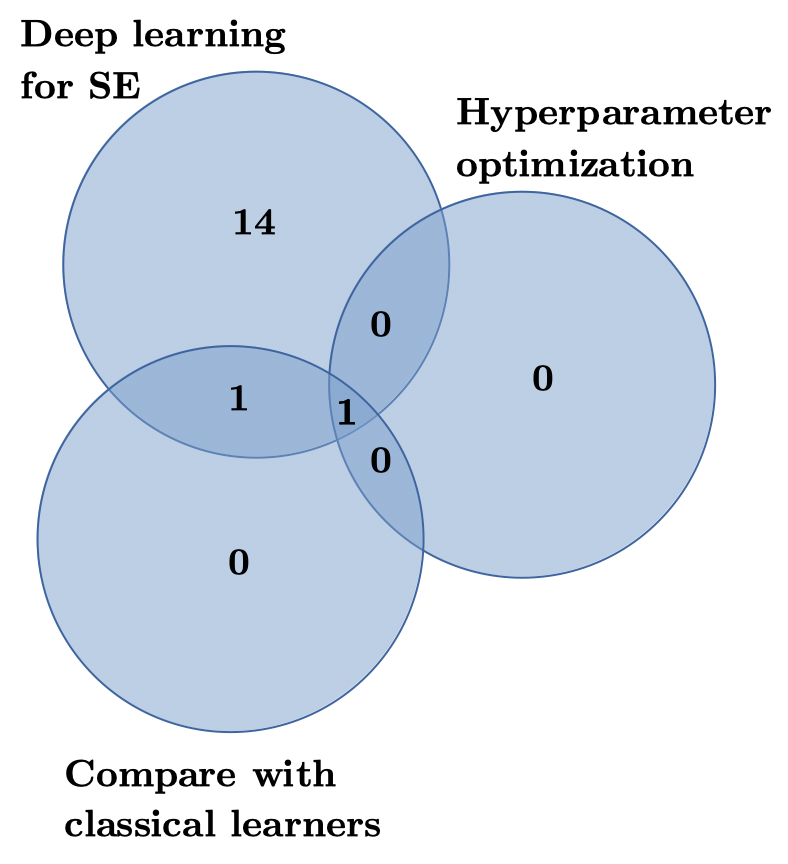
\includegraphics[width=.5\linewidth]{venn.png}
       \end{center} 
    \caption{Summary of Table \ref{tab:papers}. The paper satisfying all three criteria is \cite{wang2016automatically}; the paper that compares with classical learners is \cite{dam2019lessons}}
    \label{fig:venn}
\end{figure}
One  feature we note from our sample of research papers
 is that the code and data for most of the these papers is not always open source. Some are even protected by patent applications. This has implications for reproducibility. For example, 
 this paper
 baselines
 some of our
 results against
  Wang et al. \cite{wang2016automatically}.
  Their methods
  are protected by a patent, and therefore we could not replicate their results using their code.
  That said, we were able to 
  find their exact training and test sets,
  which we used
  for comparison purposes.
 
 Figure \ref{fig:venn} summarizes key features of that literature. 
 Note that few papers compare their results with non-deep learning methods \cite{wang2016automatically,dam2019lessons}. Also, 
Figure~\ref{fig:venn} shows only one prior
result which included deep learning, hyperparameter optimization, and a comparison to non-DL methods~\cite{wang2016automatically}. 
Further,
Several of the papers warn of the extreme   cost of performing deep learning; specifically, very long training times 
(e.g. when learning semantic features~\cite{wang2016automatically}).
Furthermore,
most of the papers do not perform a structured hyperparameter optimization (we only see this done by \cite{wang2016automatically}, using a grid search approach). Even then, very few hyperparameters are tested.

 
\begin{table*}[!t]
% \caption{Learners and preprocessors used by DODGE and GHOST}
% \label{tab:dodge}
%\captionsetup{font=footnotesize}

\scriptsize
 
 \begin{tcolorbox}[colback=white]
 \begin{flushleft}
\textbf{Learners used by DODGE:}  

\noindent
\begin{itemize}
\item DecisionTreeClassifier(criterion=b, splitter=c, min\_samples\_split=a).
    a, b, c= randuniform(0.0,1.0), randchoice([`gini',`entropy']),   randchoice([`best',`random']).
  
\item RandomForestClassifier(n\_estimators=a,criterion=b,  min\_samples\_split=c).  a,b,c = randint(50, 150), randchoice(['gini', 'entropy']),  randuniform(0.0, 1.0) 
 
\item LogisticRegression(penalty=a, tol=b, C=float(c)).
       a,b,c=randchoice([`l1',`l2']), randuniform(0.0,0.1), randint(1,500)
     
\item MultinomialNB(alpha=a) = randuniform(0.0,0.1)
\item KNeighborsClassifier(n\_neighbors=a, weights=b, p=d, metric=c).  a, b,c  = randint(2, 25), randchoice([`uniform', `distance']),  randchoice([`minkowski',`chebyshev']). 
  If c=='minkowski': d= randint(1,15)  else:  d=2

\end{itemize}


{\bf Pre-processors used by DODGE (and the ones in italics were also used  by GHOST):} 

\bi 
\item \textit{StandardScaler}
\item \textit{MinMaxScaler}
\item \textit{Normalizer(norm=a) = randchoice([`l1', `l2',`max'])}
 \item MaxAbsScaler
 \item RobustScaler(quantile\_range=(a, b)) =  randint(0,50), randint(51,100) 
 \item KernelCenterer
 \item QuantileTransformer(n\_quantiles=a,  output\_distribution=c, subsample=b). a, b = randint(100, 1000), randint(1000, 1e5);
   c=randchoice([`normal',`uniform']).
\item Binarizer(threshold=a) =  randuniform(0,100)
     
\ei
\end{flushleft}
\end{tcolorbox}
\caption{Hyperparameter  options explored by DODGE \cite{agrawal2019dodge}.  GHOST optimizers uses some of these parameters (see the pre-processing options shown in {\em italics}) in the manner discussed in Table~\ref{tab:preprocessors2}.}\label{tab:preprocessors1}
\end{table*}



 This lack of hyperparameter optimization in DL defect prediction  papers~\cite{wang2016automatically,dam2019lessons, wang2018deep}
is of some concern.
Hyperparameter optimization is the tuning of so-called ``hyperparameters"--parameters that are not learned by the algorithm, but instead drive the working of the algorithm--to attain optimal performance.  
Hyperparameter optimization is very useful when using complex   learners.
This is especially true for deep learners, which have exponentially more parameters and complex loss surfaces to explore. Montufar et al. ~\cite{montufar2014number} note that the expressive power of deep learners comes from the architecture, which determines bounds on the number of piecewise linear regions that can be represented as a decision boundary.


\subsection{Hyperparameter Optimization}

% Our paper stands out from the above papers by addressing these claims. Specifically, we 
% \begin{itemize}
%     \item Compare against results that use hyperparameter optimization on classical machine learning models.
    
%   \item Perform hyperparameter optimization on a larger set of hyper-parameters, and use baselines based on the recommendations of deep learning literature \cite{montufar2014number}.
%     \item   We   show that, at least for these data sets, such tuning is not very computational expensive. 
%     For example,  our approach takes less than 4 minutes to train a neural network.

%         \item Make our code and data open source to promote the open science in software engineering.
%             This is important since, in the above survey, we found that only three of the above seventeen papers \cite{hoang2019deepjit,Tufano2018,choetkiertikul2018deep} have
%     made public the scripts and data used in their work.  
% \end{itemize}




Hyperparameter optimization  is
the automatic tuning
of many parameters that control the internal settings of the learner and data preprocessors.
The last 15 years have seen a dramatic
increase in the application of machine learning and hyperparameter optimization (HPO)
 to software analytics~\cite{menzies2003data,last2003data,moeyersoms2015comprehensible,menzies2018software,kim2016emerging,menzies2006data,robillard2009recommendation,hassan2008road}.
% With modern hardware becoming increasingly powerful and computational power cost decreasing, the use of more computationally expensive models is becoming more feasible. Yet, many deep learners are still too expensive to run, and therefore there is a need for cheaper, better defect predictors.
% Deep learnering can be a very slow process. For example, the smallest ResNet \cite{he2016deep}
% (ResNet50) has 25 million parameters while other versions (e.g. DenseNets~\cite{huang2017densely}) have upwards of 8 million parameters (e.g.   the recent GPT-3  model \cite{brown2020language} have over 175 billion parameters). However, the complex architectures used for image and language data are not required for software, where the data is intrinsically simple. Therefore, we train simple deep learning models, with few layers, and only densely connected layers, using recommendations from \cite{montufar2014number}.
% This is an important technique since
% numerous researchers reported that data making and data pre-processing techniques/algorithms/tools are often used in a ``black box'' manner without reflecting on
% the merits of choices associated with a particular   tool~\cite{fu2016tuning,Binkley:2018}.
% Such black-box usage is risky since it
% means   SE practitioners might be  applying the wrong tool. Hence,
% An emerging question in the application of machine learning techniques to software engineering is the
% validity of the assumptions that underlie the creation of those tools and techniques. 
% Numerous
% researchers now ask if 
% superior results can be obtained by adapting
% machine learning tools   to the particulars of software engineering problem~\cite{Binkley:2018,fu2016tuning,agrawal2018better,tantithamthavorn2016automated,Novielli:2018}.  
A repeated results is that 
research results    from an ``off-the-shelf'' learner might be overturned by a second study that
tunes the hyperparameters of that learner~\cite{agrawal2019dodge}.  For example, in 2008, Lessmann et al.~\cite{Lessmann08} argued that for defect prediction, the best and worst learning methods were random forests and CART, respectively.
In 2016, Fu et al.~\cite{fu2016tuning} showed that hyperparameter optimization effectively
reverses that conclusion since  after tuning,
CART   out-performed random forests.

 
While automatically tuning various hyperparameters is rare in the SE deep learning literature (see  Figure \ref{fig:venn}),  it has been explored in other domains.
For example,   ``AutoML" methods seek the best combination of preprocessors and hyperparameters for a given dataset. These are typically based on Bayesian optimization, as in \cite{feurer2015efficient,thornton2013auto}. However, while Bayesian optimization in practice does find an optimal set of hyperparameters for deep learners, it takes a long time to run. For example, Feurer et al.~\cite{feurer2015efficient} report Auto-Sklearn results after 48 hours of running on a CPU farm.

Yet another branch, called Neural Architecture Search, also typically uses Bayesian optimization. These techniques aim to find the optimal learner architecture. These techniques have achieved a rather high level of sophistication: for example, Liu et al.~\cite{liu2019auto} describe a hierarchical approach for building neural network architectures. Elsken et al.~\cite{elsken2018neural} provide a review of neural architecture search methods. Some of these neural architecture search papers inevitably overlap with hyperparameter tuning \cite{bergstra2013making,domhan2015speeding,saxena2016convolutional,shahriari2015taking,stanley2002evolving}. 

Both these approaches share the same  concerns (a) they have long runtimes (b) some neural architecture search approaches tend to generate overly complex architectures for a problem, which may be overkill for software engineering. 
Accordingly, the rest of this paper discusses experiments with  DL hyperparameter optimization via our GHOST tool. We prefer GHOST  over
other methods since it is simple to implement, it runs quickly, and it scales to larger data sets. 

 


  
% Hence, using that tool we can show hyperparameter optimization for defect prediction is both effective and fast enough for use in practice.



\begin{table}[!b]
    \centering
    \scriptsize
    \caption{Tuning parameters for DL (used by GHOST)}
    \begin{tabularx}{\linewidth}{rp{2.5cm}L} 
        Preprocessor & Description & Options \\
        \midrule
         \texttt{StandardScaler} & Transforms the dataset to have a mean 0 and variance 1 & None \\
        \rowcolor{blue!10} \texttt{MinMaxScaler} & Squeezes the data to the range $[0,1]$. & None \\
        \texttt{Normalizer} & Normalizes samples to a unit norm. & Choice of norm: $l_1$, $l_2$,   $l_\infty$ \\
        
          \rowcolor{blue!10}  \texttt{NumLayer}s & & 1 .. 5\\
       \texttt{UnitsPerLayer} & &  2 .. 20\\
      \rowcolor{blue!10}  \texttt{Epochs} & number of times data reapplied to the algorithm & 10 .. 30\\
      \texttt{Network} & topology & Feed forward\\
       \rowcolor{blue!10} \texttt{Activation} & hidden units: & rectified linear units  \\
        \rowcolor{blue!10}                     & last layer & sigmoid\\
       
        
    \end{tabularx}
    \label{tab:preprocessors2}
\end{table}

  Table~\ref{tab:preprocessors1} and Table~\ref{tab:preprocessors2} lists    hyperparameters  that can control the algorithms that generate
defect predictors.  Table~\ref{tab:preprocessors1}, these options were collated from the hyperparameters
explored in recent SE papers~\cite{ghotra2015revisiting,fu2016tuning,agrawal2018better,agrawal2018wrong} and in  the documentation of a widely-used data mining library
(Scikit-learn~\cite{scikit-learn}).


As to Table~\ref{tab:preprocessors2}, these options come from recent papers on deep learning.
After reading the literature looking for a ``standard DL architecture'', we 
use standard feed-forward neural networks with ReLU activation functions (rectified linear units; a.k.a. ``hockey sticks'') in the hidden layers and sigmoid activation in the last layer.
As to other details of our deep learners, 
 Montufar et al. ~\cite{montufar2014number} discuss   feed forward neural networks with ReLU activations.
 The bounds for the number of piecewise linear regions constituting a decision boundary that can be represented by a deep learner, providing a proof based on topological folding.  After,  Montufar et al.,  we use no more than 3 layers with up to 20 units.
 
 One options within deep learning is how many ``epochs'' to apply (and one epoch is one run over all the data to adjust entwork weights). 
For our experiments, we used  ten epochs since,   as shown in Figure~\ref{fig:convergence}, we found very little improvement after  after five epochs
 (aside:   and in experiments with up to 256 epochs, we found little improvements over the results shown in Figure~\ref{fig:convergence}).
 



  
%  Based on the results of Santurkar et al. ~\cite{santurkar2018does}, 
% we do not use batch N=normalization \cite{ioffe2015batch} 
% since Santurkar argues th. at this for complex problems, this  flattening the loss surfaces (more precisely, it reduces the L-Lipschitzness and the $\beta$-smoothness of the loss surface), making optimization easier for gradient descent. 
 
 
%  In detail, when the number of units in any hidden layer is less than the number of inputs, the lower bound vanishes--this provided us with an upper bound for the number of units per layer (informally, while the network is still certainly capable of learning a complex decision boundary, it is no longer obliged to). To elaborate on this line of reasoning, given the results of their paper, it is trivial to show that an ideal neural network would have several layers, each with the same number of units (which in turn, is the same as the number of inputs)--this can be derived via a greedy algorithm that adds layers $l_i$ with the number of units as the number of inputs (denote this as $n_0$), until the remaining number of units (which can be trivially found from the results of the paper) is less than $2n_0$; at this point, we add one layer with the remaining number of units. While adding more units in the hidden layers certainly adds computational power, the formula presented in the paper suggests that deeper networks (in deep learning literature, ``deeper" denotes more layers) are preferable to ``wider" networks (which in deep learning literature refers to networks with more units in each layer). 



\subsubsection{Optimization with DODGE}
\label{sec:dodge}

One key point to observe from those tables is the size of optimization space. If each numeric range is divided into five bins using {\em (max-min)/5}, then Table~\ref{tab:preprocessors1} holds nine binary choices and 18 options with five choices; i.e. \[5^{18}*2^9 \approx 2*10^{15} = 2,000,000,000,000,000\;\mathit{options}\]
This space is too large to be exhaustively explored. Hence
GHOST   and 
DODGE \cite{agrawal2019dodge} explore this space heuristically.
DODGE's exploration is defined around
 a concept called $\epsilon$-domination.  Proposed by Deb in 2005~\cite{deb2005evaluating}, $\epsilon$-domination states that there is little point in optimizing two options if their performance differs by less than some small value $\epsilon$.
 
 

\begin{figure}
    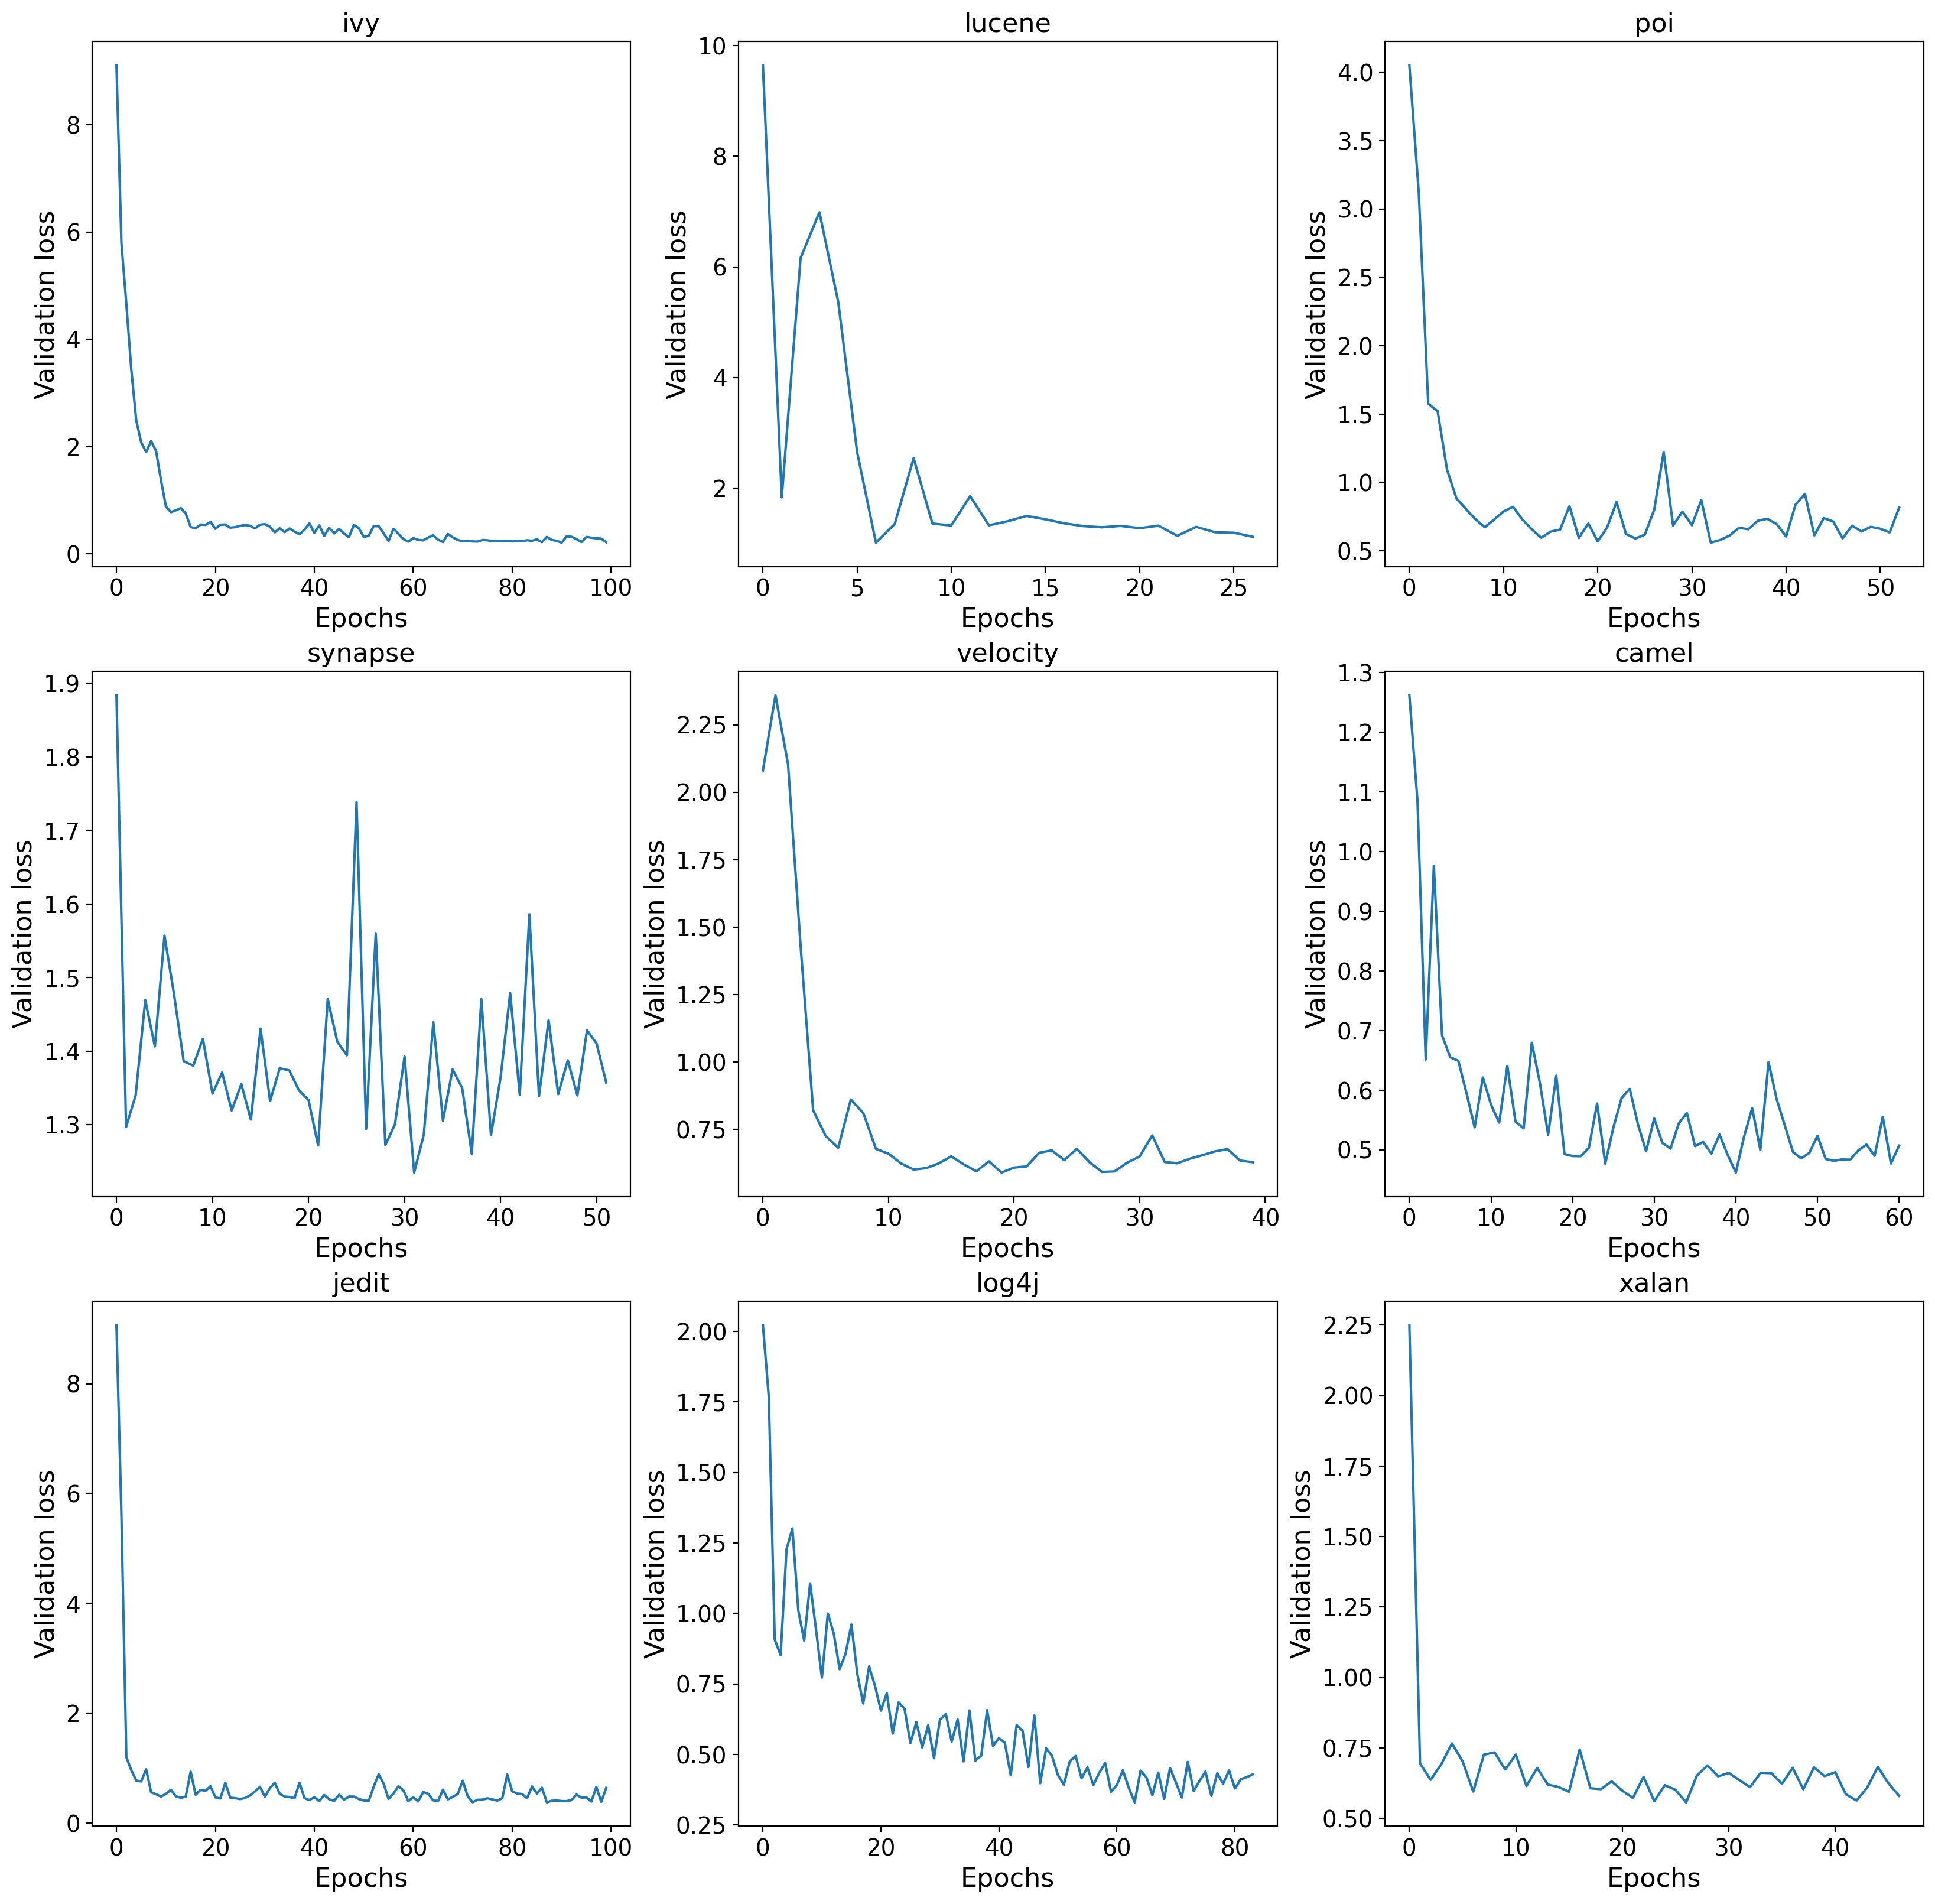
\includegraphics[width=.49\textwidth]{convergence.png}
    \caption{DL convergence on defect prediction data sets}
    \label{fig:convergence}
\end{figure}
DODGE  exploits   $\epsilon$-domination as follows. $N$ times do: (a)~generate configurations   at random, favoring those those with lowest weight (initially, all options have a weight $w=1$); (b)~if one option generates results within $\epsilon$ of some other, then   increases these options' weights (thus  decreasing the odds that they will be explored again).
This approach can be a very effective way to explore a large space 
of options.
If we assess a defect predictor  on $d=2$
dimensions (e.g. recall and false alarm), the output space of that performance divides into $(1/\epsilon)^d)$ regions.

To understand the practical implications of this,
we note that
defect predictors can exhibit a large variance
in their output, particularly for data sets like
those in Table \ref{tab:datasets} (where the size of the target class in the training and test
data  is so variable).
 Assuming  $d=2$ and $\epsilon=0.2$ then 
 our defect predictors have
$(1/0.2)^2=25$ output regions. 
Each time we apply
DODGE's tabu search, then two of these regions can  be removed; i.e. in theory, DODGE could terminate very quickly.

Agrawal et al.~\cite{agrawal2019dodge}  found that, for defect prediction,
 the optimizations found above $N=30$ repeats of
the above loop performed no worse than those found after $N=1000$ loops. Better yet, the optimizations found that way
out-performed numerous prior results.

\subsubsection{Optimization with GHOST}
The lesson of DODGE is that the particulars
of Table~\ref{tab:preprocessors1} can be
less important than how we explore combinations
of learning methods.   So can we do more with
that insight? Is there some process more
direct that DODGE that explores, in a
more direct way, how to divide data
into regions that (e.g.) do or do not
predict for defects?

This section proposes GHOST as an
answer to those questions. To understand
GHOST, we first take a glance at   our defect prediction data. Table~\ref{tab:attributes} shows
the static code attributes seen in our data
and Table~\ref{tab:datasets} shows what releases
we use for our training and test sets when comparing with DODGE\footnote{These releases were selected as follows: in the available data, use recent releases to predict for defects in the latest release.} (when comparing against our other baseline by Wang et al. \cite{wang2018deep}, we use the same train and test release versions as they do). A curious feature of    Table~\ref{tab:datasets} is the wide variability in the percent of defects seen in the training and test sets. For example, the defect ratios in: 
\bi
\item  velocity's  train:test ratios decrease from 71 to 34\%;
\item jEdit's train:test sets ratios decrease from  23 to 2\%;
\item xerces' train:test sets ratios increase from  16 to 74\%.
\item log4j's train:test sets ratios increase from  29 to 92\%;
\item xalan's train:test sets ratios increase from 38 to 99\%;
\ei
Such massive changes in the target class ratios means
that the geometry of the hyperspace boundary
between different classifications  
can alter dramatically between train and test.
Therefore, the ``appropriate
learner''   for
this kind of data is one that
works well for a wide range
of ratios
of class distributions.
Such an appropriate learner
knows how to exploit
``hints'' from the hyperspace boundary in the train
set, then apply those hints to the test set.

GHOST was  implemented as an experiment
to see if the   {\em loss functions} of neural networks can learn such ``hints''.
What the rest of this paper   shows is that
 such loss function
 (plus some
fuzzy oversampling, described below) is an effective
method for handling defect prediction.

\subsubsection{Loss Functions}
\label{sec:loss}
In neural networks, the loss function is the prediction error seen in the last epoch of the
neural net. The loss is used to calculate the gradients used to  update the weights of the neural net for the next epoch of learning. 
Loss can be calculated in various ways\footnote{ 
mean squared error,  
binary crossentropy, 
categorical crossentropy,
sparse categorical crossentropy, etc. } but the key point to note here is that, usually, the loss function is fixed prior to learning.



\begin{table}
    \centering
    \caption{Static attributes in our  datasets.}
    \begin{tabularx}{\linewidth}{lL}
    \toprule
        Attribute   & Description (with respect to a class) \\
        \midrule
        wmc & Weighted methods per class \cite{chidamber1994metrics} \\
    \rowcolor{blue!10}    dit & Depth of inheritance tree \cite{chidamber1994metrics} \\
        noc & Number of children \cite{chidamber1994metrics} \\
    \rowcolor{blue!10}    cbo & Coupling between objects \cite{chidamber1994metrics} \\
        rfc & Response for a class \cite{chidamber1994metrics} \\
    \rowcolor{blue!10}    lcom & Lack of cohesion in methods \cite{chidamber1994metrics} \\
        lcom3 & Another lcom metric proposed by Henderson-Sellers \cite{henderson1996coupling} \\
    \rowcolor{blue!10}    npm & Number of public methods \cite{bansiya2002hierarchical} \\
        loc & Number of lines of code \cite{bansiya2002hierarchical} \\
    \rowcolor{blue!10}    dam & Fraction of private or protected attributes \cite{bansiya2002hierarchical} \\
        moa & Number of fields that are user-defined types \cite{bansiya2002hierarchical} \\
    \rowcolor{blue!10} mfa & Fraction of accessible methods that are inherited \cite{bansiya2002hierarchical} \\
        cam & Cohesion among methods of a class based on parameter list \cite{bansiya2002hierarchical} \\
    \rowcolor{blue!10} ic & Inheritance coupling \cite{tang1999empirical} \\
        cbm & Coupling between methods \cite{tang1999empirical} \\
    \rowcolor{blue!10} amc & Average method complexity \cite{tang1999empirical} \\
        ca & Number of classes depending on a class \cite{tang1999empirical} \\
    \rowcolor{blue!10} ce & Number of classes a class depends on \cite{tang1999empirical} \\
        max\_cc & Maximum McCabe's cyclomatic complexity score of methods \cite{mccabe1976complexity} \\
    \rowcolor{blue!10} avg\_cc & Mean of McCabe's cyclomatic complexity score of methods \cite{mccabe1976complexity} 
    \end{tabularx}
    \label{tab:attributes}
\end{table}


\begin{table} 
    \centering
    \caption{Evaluated software projects for comparing with DODGE \cite{agrawal2019dodge}}
    \begin{tabularx}{\linewidth}{lllLL}
        \toprule
        Project & Train versions & Test versions & Training Buggy \% & Test  Buggy \% \\
        \midrule
        ivy & 1.1, 1.4 & 2.0 & 22 & 11 \\
        \rowcolor{blue!10} lucene & 2.0, 2.2 & 2.4 & 53 & 60 \\
        poi & 1.5, 2.0, 2.5 & 3.0 & 46 & 65 \\
        \rowcolor{blue!10}synapse & 1.0, 1.1 & 1.2 & 20 & 34 \\
        velocity & 1.4, 1.5 & 1.6 & 71 & 34 \\
        \rowcolor{blue!10}camel & 1.0, 1.2, 1.4 & 1.6 & 21 & 19 \\
        jEdit & 3.2, 4,0, 4.1, 4.2 & 4.3 & 23 & 2 \\
        \rowcolor{blue!10}log4j & 1.0, 1.1 & 1.2 & 29 & 92 \\
        xalan & 2.4, 2.5, 2.6 & 2.7 & 38 & 99 \\
        \rowcolor{blue!10}xerces & 1.2, 1.3 & 1.4 & 16 & 74 \\
        \bottomrule \\
    \end{tabularx}
    \label{tab:datasets}
\end{table}



\begin{figure}[!h]
\centering
    \begin{subfigure}[b]{.4\textwidth}
        \centering
        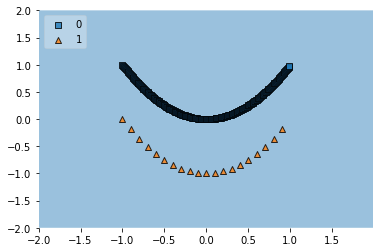
\includegraphics[width=.7\textwidth]{unweighted.png}
        \caption{Unweighted loss function}
        \label{fig:unweighted}
    \end{subfigure}
    %
    \begin{subfigure}[b]{.4\textwidth}
        \centering
        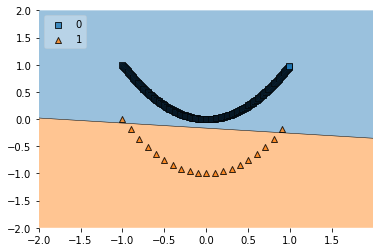
\includegraphics[width=.7\textwidth]{weighted.png}
        \caption{Weighted loss function}
        \label{fig:weighted}
    \end{subfigure}
    \caption{The two arcs in these figures show points selected from two distributions: $y_1=x_1^2$ and $y_2=x_1^2-1$ (where $y_1$ is ten times more frequent than $y_2$).  The background colors show the hyperspaces learned by a neural network. Note that, in the top plot (using an unweighted loss function), the hyperspace is all one color; i.e, it does not distinguish between the two populations. But in the lower plot, the hyperspace divided into blue and orange, where orange denotes the region where the neural net predicts that the data comes from the minority  $x_1^2-1$. distribution. Observe how  the unweighted loss function misses all the minority class with  while the  weighted loss function can find nearly all  of the minority class.}
\end{figure}

In 2019, Cui et al.~\cite{Cui_2019_CVPR} proposed dynamically adjusted loss functions that know how to adjust the loss function in order to reduce the overlap between sets of positive and  negative examples.
Their re-weighting scheme   uses the effective number of samples for each class to re-balance the loss, thereby yielding a class-balanced loss. Their experiments show that,
when trained with a dynamic class-balanced loss function, the network is able to achieve significant performance gains on data sets with class imbalance. 

The methods of  Cui et al. assumed high dimensional vision data (with, sometimes, over 8000 classes), so we can  not  directly apply their methods here. However, inspired by their work, we did design a class balance method that proved to be effective for defect prediction.
To illustrate that method, we artificially generated two sets of data with very different class distributions. This data had 200 rows and three columns:
\bi
\item A class column, whose values are selected at random, with the negative class being 10 times more likely than the positive class)

\item
Two other columns which we call $x_1, x_2$
where $x_1$ is selected  randomly -1 to 1
and $x_2$ is
\bi
\item For the negative examples,  $x_2=x_1^2$;
\item For the positive examples $x_2=x_1^2-1$.
\ei
\ei
We then ran a deep learner (with one hidden layer) for 10 epochs, with and without the weighted loss function (described below).
Figures \ref{fig:unweighted} and \ref{fig:weighted} show the results. 
Observe how,
with an unweighted loss function, the neural network completely ignores the positive class, but with the weighted version, it recognizes the importance of the positive examples, pushing the accuracy up from 90.91\% to 99.09\%. 

\BLUE
\subsubsection{Notation used}
\label{sec:notation}
We briefly discuss notation used in Algorithm \ref{alg:ghost} for clarity:  \respto{2a6.1}
\begin{itemize}
    \item we use $f(\textbf{x}; \theta)$ to denote a neural network $f(\cdot)$;
    \item we denote inputs by $\textbf{x}$ (we do not require a subscript to denote index since individual points are not referenced;
    \item the neural network function above is \textit{parameterized by} the hyperparameter (and preprocessor) set $\theta$;
    \item we use $\hat{\textbf{y}}$ to denote the predicted values and $\textbf{y}$ to denote the true values;
    \item we use $\hat{\mathcal{L}}$ to denote our modified loss function
    \item we use $m$ to denote the number of training samples;
    \item we use $n$ to represent the ratio of majority class samples to minority class samples (so that $n > 1$);
    \item without loss of generality, we use $c_0$ to denote the minority class, and $c_1$ to denote the majority class;
\end{itemize}
\BLACK
 
%  the answer is fairly clear: deep learners off the shelf are not tuned for specific metrics. Even when tuned for accuracy, deep learners will sometimes find ``easy", suboptimal solutions (as in Figure \ref{fig:unweighted}), and need to be pushed towards better solutions by biasing the loss function. Our motivation for using such weighted loss functions based on this example is by noting that defect prediction datasets have a class imbalance problem (see Table \ref{tab:datasets}), where the buggy modules are underrepresented. The biases applied are not necessarily non-trivial--by simply adjusting the weight, it is possible to bias learners towards specific goals.

We now elaborate on the weighted loss functions used in
Figure~\ref{fig:weighted}.  Consider a loss function $\mathcal{L}(y, \hat{y})$ (where $y$ is a vector representing the target outputs, and $\hat{y}$ is a vector representing the predictions) optimized by a neural network. As is the case with defect prediction, consider the case of binary classification. Let $c_0$ be the minority class, and $C$ be the set of all classes; for binary classification, this is simply the set $\{c_0, c_1\}$. Denote a training example by a subscript (i.e., let $y_i$ denote the target of the $i$th training example), and let $m$ be the number of training examples. Then, the loss function can be rewritten as:

% \begin{align}
%     \mathcal{L}(y, \hat{y}) &= \sum_{i=1}^m \mathcal{L}(y_i, \hat{y_i}) \nonumber \\
%     &= \sum_{\substack{i=1 \\ y_i = c_0}}^m \mathcal{L}(y_i, \hat{y_i}) + \sum_{\substack{i=1 \\ y_i \neq c_0}}^m \mathcal{L}(y_i, \hat{y_i})
% \end{align}



\[
    \begin{aligned}
    \mathcal{L}(y, \hat{y}) &= \sum_{i=1}^m \mathcal{L}(y_i, \hat{y_i}) \nonumber = \sum_{\substack{i=1 \\ y_i = c_0}}^m \mathcal{L}(y_i, \hat{y_i}) + \sum_{\substack{i=1 \\ y_i \neq c_0}}^m \mathcal{L}(y_i, \hat{y_i})
    \end{aligned}
\]
We call the above the \textit{unweighted} loss function. Now, we apply a fairly obvious method of weighting the above as follows. Let $n$ be the fraction of samples with class $c_0$. Then, we re-weight the loss function above to:

\begin{equation}\label{eq:w}
\begin{aligned}
    \mathcal{L}^1(y_i, \hat{y_i}) &= \frac{w_i}{n}\sum_{\substack{i=1 \\ y_i = c_0}}^m \mathcal{L}(y_i, \hat{y_i}) + \sum_{\substack{i=1 \\ y_i \neq c_0}}^m \mathcal{L}(y_i, \hat{y_i})
    \end{aligned}
\end{equation}
where $w_i$ is the weight control parameter. For this study, we ran with   various  weights  $w_i  \in \{1,10,100\}$ and found no appreciable difference between these settings. Hence, in the following, we use $w_i=1$. As an aside, we note that this can be extended to multi-class classification in several ways, one of them being adapting each $w_i$ so that the effective number of samples of each class ($\frac{w_i}{n_i}$) is roughly the same (this can be done using the lowest common multiple of the number of samples in each class).


Clearly, as the minority class shrinks, there is a greater emphasis placed on getting these data points right. This is similar to oversampling by $\frac{w_i}{n}$ because with the unweighted loss function and oversampled data, an individual minority class data point (now represented multiple times) contributes more to the loss function than a majority class data point. However, using a weighted loss function has several advantages (a) we do not need to load additional samples into memory (b) we save computation since we do not need to run iterations over these samples (c) it is flexible: we can use a different weight easily.

 We certainly are not the first to attempt a reweighted loss function: Lin et al.~\cite{lin2017focal} propose a ``focal loss" function that uses an exponential weighting scheme. However, to the best of our knowledge, we are the first to apply this with various weights in the software engineering domain.


\subsubsection{Weighted Fuzzy Oversampling}
\label{sec:wfo}

We found experimentally that while using a weighted loss function does improve performance, we can do better still, through weighted fuzzy oversampling. This is motivated by a desire to achieve more ``robust" decision boundaries. Let $\gamma_i$ be the (shortest) distance from a minority sample to the decision boundary. Akin to the terminology used in support vector machines, we call $\gamma_i$ the \textit{functional margin}, and $\gamma = \min\limits_i \gamma_i$ the \textit{geometric margin}. Our proposed weighted fuzzy oversampling is motivated by the SVM goal to achieve $\hat{y} = w^Tx + b \geq \gamma$. 
% SVMs  impose a scaling constraint to ensure a convex optimization problem; since the loss surfaces of deep learners are generally non-convex (for a detailed discussion, see \cite{santurkar2018does}), we find this unnecessary. For the same robustness reasons that SVMs maximize the geometric margin, the use of weighted fuzzy oversampling is motivated by a desire to build robust decision boundaries by increasing each functional margin (and therefore, the geometric margin). In particular, we note that while weighted loss functions motivate the deep learner to learn decision boundaries that consider the minority class, it has no obligation to learn a ``robust" boundary. 
Using the same notation as the weighted loss functions, let $n$ represent the fraction of samples in the minority class $c_0$. Then, iteratively, we add the training samples $(\textbf{x} - i \boldsymbol{\Delta r}, c_0)$ and $(\textbf{x} + i\boldsymbol{\Delta r}, c_0)$ for each sample $(\textbf{x}, c_0)$ in the minority class. At iteration $i$, we add the new samples $\frac{(1 / n)}{2^i}$ times; we iterate till this value is 0. Here, $\boldsymbol{\Delta r}$ (which we note is a vector) is a user-specified parameter; in our experiments, we found that values between 0.01 and 0.05 work well. We note here that it might be more beneficial to choose $\Delta r$ based on the statistics of each attribute, but we do not explore that here. Algorithm \ref{alg:wfo} describes weighted fuzzy oversampling.

\begin{algorithm}[h]
\footnotesize
    \SetAlgoLined
    \For{each sample $\textbf{x}$ in the minority class}{
        \For{$i$ such that $\frac{(1/n)}{2^i} >= 1$}{
            Add $(\textbf{x} \pm i\Delta r, c_0)$ to the training set\;
        }
    }
    \caption{Weighted fuzzy oversampling}
    \label{alg:wfo}
\end{algorithm}



\begin{algorithm}[!h]
\footnotesize
    \SetAlgoLined
    Separate the data into train and test sets\;
    Apply weighted fuzzy oversampling to the training set\;
    Apply SMOTE to the resulting training set\;
    Choose a set of key hyperparameters and pre-processors\;
    Build a list of options for preprocessing and tuning, and assign every node a weight of 0\;
    Sample at random to create random combinations of preprocessors and hyperparameters\;
    \For{$N_1$ random samples $\theta_1,\ldots,\theta_{N_1}$}{
        \For{$N_0$ epochs}{
            $\hat{\textbf{y}} = f(\textbf{x}; \theta_i)$\;
            $\textbf{w} = \textbf{w} - \nabla_{\textbf{w}} \hat{\mathcal{L}}(\textbf{y}, \hat{\textbf{y}})$\;
        }
        $\phi_i = \text{eval}(f)$\;
    }
    \For{options that result in metrics with a difference $<\epsilon$} {
        Reduce the weight by 1\;
    }
    \ForAll{other options}{
        Increase the weight by 1\;
    }
    \For{$N_2$ evaluations}{
        Choose the options with the highest weight, and mutate its parameter settings\;
        \For{$N_0$ epochs}{
            $\hat{\textbf{y}} = f(\textbf{x}; \theta_i)$\;
            $\textbf{w} = \textbf{w} - \nabla_{\textbf{w}} \hat{\mathcal{L}}(\textbf{y}, \hat{\textbf{y}}$)\;
        }
        $\theta^* = \text{argmax}_{\theta} \text{eval}(f)$\;
    }
    \KwRet{$\theta^*$}
    \caption{GHOST}
    \label{alg:ghost}
\end{algorithm}


\subsubsection{Pseudo-code}
\label{sec:pseudocode}
As shown in  Algorithm \ref{alg:ghost}, 
GHOST uses weighted loss functions (lines 10,24),
 DODGE's    ``$\epsilon$-domiantion'' (line 14), and
   weighted fuzzy oversampling (line 2).
    Having tuned the deep learner to (a) learn to recognize the minority class and (b) learn robust decision boundaries using the above methods,
    we found that
    GHOST achieved good recalls, but the learners now have trouble recognizing the negative examples, due to the minority class being \textit{over-oversampled}. We fix this using SMOTE~\cite{Chawla02} with the default settings.
   SMOTE is a method for handling class
    imbalance. In the training set, this algorithm discards instances
    from the majority class while also generating
    artificial examples of the minority class (by extrapolating between near neighbors of the same class).

\BLUE
Weighted loss functions perform standard oversampling in a computationally efficient way, balancing out the classes. However, it achieves this efficiency by weighting each minority class sample more. Therefore, the deep learner can, in theory, still reduce the value of this loss function by narrowly classifying the minority samples correctly. This behavior is undesired because it is, essentially, overfitting on part of the learner, since it only adjusted the decision boundary based on the training data. Weighted fuzzy oversampling is an attempt to alleviate this issue by adding ``guard points" around the minority class point, further pushing away the neural network decision boundary. That said, we do not wish to ``pollute" the original training data with fake data points, and so we reduce the ``value" (where value means the loss function value) of these points with the exponential decay (the $2^i$ in the denominator).

Finally, with the extra added points, the data is now unbalanced the other way, and we fix this with a well-known oversampling strategy, SMOTE.
\respto{1a3.1}
\BLACK

(Technical aside:  SMOTE is different from weighted fuzzy oversampling-- while SMOTE adds one point randomly between one of $k$ nearest neighbors, weighted fuzzy oversampling radially oversamples points with an exponentially decaying weight.)





%The first two lines of  Algorithm \ref{alg:ghost} are standard among all learning tasks.
%Lines 3 and 4 are taken from  DODGE: we maintain a set of hyperparameter and preprocessor settings, and assign them an initial weight of 0. This weight is modified in lines 13 and 16 if they lead to similar performance (according to the goal criteria): if the difference in performance is less than $\epsilon$, we do not pursue them further and reduce their weight. The authors of DODGE claim that different values of $\epsilon$ lead to the same result; therefore, we use $\epsilon = 0.2$. 

%In lines 5-11, we evaluate $N_1$ random samples among the candidate pool. As suggested by the authors of DODGE, we use the default value $N_1 = 12$. The evaluation consists of training a deep learner with the current hyperparameter choice (lines 6-9), and calling an \texttt{eval} function that  runs forward propagation on the test set and evaluates the learner according to the metric of choice. Finally, for $N_2=30$ (default value) evaluations, we mutate the highest weighted hyperparameter set and evaluate it, keeping track of the best set of hyperparameters (which we call $\theta^*$).

% We briefly discuss notation used in Algorithm \ref{alg:ghost} to clarify any confusion: we use $f(\textbf{x}; \theta)$ to denote a neural network $f(\cdot)$, whose inputs are $\textbf{x}$, \textit{parameterized by} the hyperparameter (and preprocessor) set $\theta$. We use $\hat{\textbf{y}}$ to denote the predicted values and $\textbf{y}$ to denote the true values. Finally, we use $\hat{\mathcal{L}}$ to denote our modified loss function.

\section{Experimental Methods}
\label{sec:method}

The rest of this paper
discusses a comparative evaluation
of GHOST with DODGE, standard deep learning, and the results of Wang et al. \cite{wang2018deep}, who use a Deep Belief Network \cite{hinton2009deep}.



\subsection{Experimental Design}

Our experiments  compared different defect predictors. For non-DL learners, we used the  methods from DODGE \cite{agrawal2019dodge}.


 For DL learning, we adopted a deep learner with 4 layers and 20 units per layer, trained for 10 epochs (from Theorem 5 in Montufar et al. \cite{montufar2014number}) We choose this based on the results of their paper, which was published in a top machine learning conference (NeurIPS 2014). While some deep learning researchers might be surprised to see that we only trained for 10 epochs, we found experimentally that this was sufficient for AUC and popt20; for recall and false alarm rate, we used 30 epochs.

 For deep belief networks (DBN), the methods seen in a TSE'18 paper  by
Wang et al. \cite{wang2018deep}. 
In that approach,
for each file in the source code, they extract tokens, disregarding ones that do not affect the semantics of the code, such as variable names. 
These tokens are vectorized, and given unique numbers, forming a vector of integers for each source file. 
These vector-buggy pairs form the training set, which are input to a Deep Belief Network (DBN), a neural network architecture designed to extract features. The extracted features are used as input to a classical learner, such as Naive Bayes. 

We    use Wang et al. since (a)~that paper made a convincing case that this approach represented a  state-of-the-art results for defect prediction for
 features extracted from source code and  (b) a deep learner is used to extract features, rather than being used as the learner, in contrast to our approach; this forms a valuable comparison.


We also explored two variants of defect prediction:
\bi
\item 
{\em Within-project defect prediction (WPDP).} Here, models
learned from earlier releases of some project  predict properties
of latter releases of that project.
\item
{\em Cross-project defect prediction (CPDP).} Here, models learned
from project1 where then applied to project2. 
\ei
To compare our results
with other cross-project methods, we used TCA+~\cite{liu2019two} since
that paper reported that TCA+ performed as well, or better, than the prior work.
We compare these against the results of GHOST. On experimenting with weights $w_i\in\{1, 10,  100\}$ (from Equation~\ref{eq:w}), we noticed no improvement over $w_i=1$. Hence, we use that weight to optimize for   each of the  performance goals
listed in \S\ref{sec:perfs}.
%: AUC, recall, false alarm rate, and popt20.  

When comparing against DODGE, in  we split the data into train and test sets, as shown in Table \ref{tab:datasets}.  GHOST used the training sets to find good DL settings, which were then applied to the test suite.


We ran our experiments on two machines:
(a) an Intel Broadwell CPU with 6 cores, 39GB RAM; and (b) a NVIDIA Tesla V100 GPU with 16 GB VRAM. The other had 15 GB RAM and a NVIDIA Tesla P100 GPU with 16 GB VRAM.
%\footnote{To justify that memory, we note that such high RAM is not necessarily required. We know this since   early versions of our code had a memory leak issue, and on fixing it, we found that 10 GB was sufficient.}.

Because of the stochastic nature of deep learning (caused by random weight initialization), a statistically valid study of its merits should consider the distribution of its performance. For this reason, we run GHOST 20 times for each dataset, for each metric. All the results reported (in Table \ref{tab:results} and Table \ref{tab:tan}) are median values of these 20 runs.

\subsection{Data}
For this study, we use the same data used in DODGE's prior study~\cite{agrawal2019dodge} on defect prediction: see Table \ref{tab:datasets}. These are all open source Java projects from  the PROMISE repository \cite{Sayyad-Shirabad+Menzies:2005}.  Each dataset has 20 static attributes for each software project, described in Table \ref{tab:attributes}.

% In our subsequent discussion, the
% following feature of  Table \ref{tab:datasets} will become very important. In this table,  the  class balance    between defective and non-defective modules is highly variable between our train and test sets:
% \bi
% \item For example,   in velocity  and jedit, the percent of defect modules decreases more than half between train and test sets;
% \item The reverse pattern is seen in the train/test sets of other data sets.
% For example,  the percentage of defect modules
% increases by (approx) 50\% (for poi and synapse) and by over 300\% (for log4j,xalan, xerces). 
% \ei
%  This feature will  motivated the design of the GHOST method, described later in this paper.





\subsection{Performance Metrics}\label{sec:perfs}
For this study, we use   performance metrics widely used     used in 
the defect predication literature.
Specifically, we evaluate the performance of our learners using three metrics: Area Under the ROC Curve (AUC) with false positive rate on the x-axis and true positive rate on the y-axis, recall, false alarm rate, and popt20. We use these measures to compare against the baseline of Agrawal et al.~\cite{agrawal2019dodge}.

Recall measures the number of positive examples that were correctly classified by a learner:

\[
    \text{recall} = \mathit{TP}\;/\;(\mathit{TP}+\mathit{FN})
\]
where TP is the number of true positives and FN is the number of false negatives.
The false alarm rate is the number of times a classifier incorrectly classifies an instance as a positive example, when it is in fact, not. Often, the false alarms observed in these experiments is very
small. Specifically, in our experiments, many of the false alarm results were 0. Hence, we will use {\em pf}, defined as follows:

\[
     \text{pf} =  \mathit{FP}\;/\;(\mathit{FP}+\mathit{TN}) %= %\frac{\text{TN}}{\text{FP}+\text{TN}}
\]
where FP is the number of false positives and TN is the number of true negatives. 

The next metric, popt20 comments on the inspection effort required after a defect predictor is run. To calculate popt20, we list the defective modules before the non-defective modules, sorting both groups in ascending order of lines of code. Charting the percentage of defects that would be recalled if we traverse the code sorted in this manner in the y-axis, we report the value at the 20\% point. 


Finally, we report the area under the receiver operating characteristics (ROC) curve (AUC), with false positive rate on the x-axis and true positive rate on the y-axis.

Note
that, with one exception,  for most of these performance measures, {\em larger} values are {\em better} since:
\begin{itemize}
\item
As  recall increases,
  more defective modules are seen.   

 \item
 As  popt20 increases, the  learner recommends that the developer inspect  smaller parts of the code (to find bugs).
 That is to say, the learner is decreasing the work load of the developer.   
  \item
  As  AUC increases, our learners  are finding more true positives and avoiding more true negatives.

\end{itemize}
The one exception is pf where {\em smaller} values are {\em better} since,
 as   pf decreases,
there are fewer cases where we waste a developer's time showing them modules which are not really defective. 

\subsection{Impact of Performance Metrics}
The original DODGE paper evaluated its models using metrics that were nuanced different to the above.
For example,
that study did not report recalls and false alarms.
When  we checked DODGE's false alarms and recalls, we found that the results depended on the optimization goals; e.g. (a)~optimizing 
 for recall  leads to higher  recalls but nearly 100\% false alarms;
(b)~optimizing  for false alarms  leads to near zero false alarms, but also near zero recalls. Hence, 
to ensure low false alarms and high recalls, our optimizers guide their search by trying to maximize the harmonic mean of high recalls $r$ and precision {\em p}; i.e. 
\[ f_1 = 2rp\;/\;(r+p)\]The results of that search were then assess via the performance measures listed in the last section.

To simplify DODGE's search (and improve its performance scores), we applied a feature selection algorithm to the data sets prior to optimization. Feature selectors
prune superfluous attributes (i.e. those not associated to the number of defects).
Following the advice of Hall and Holmes~\cite{holmes03}, we used Hall's own  CFS    selector~\cite{hall00}.

We also improved on the   nine data pre-processors used by DODGE. To address issues of class imbalance then SMOTE tool~\cite{Chawla02} down samples the majority class while  generating artificial examples of the minority class.

In summary, when we say ``DODGE'' below, we mean the original DODGE, optimizing for a specific metric, or maximizing F1 (in the case of recall and false alarm rate), after  (a)~feature selection with CFS and (b)~SMOTE. 

\subsection{Statistics}
\label{sec:stats}

The statistical methods used in this paper were selected according to the particulars of our experiments.

For example, in  the {\em within-company experiment}s,  we are using learners that employ stochastic search. When testing such algorithms, it is standard~\cite{arcuri11} to repeat  those runs 20 times with different random number
seeds. Such  experiments generate a distribution of  20 results per learner per data set.
 For those experiments, we use
 the {\em distribution  statistics} of \S\ref{sec:dist}
 to compare the efficacy
 of different learners.
 
 For the cross-company experiments, we are comparing our results against the methods of Wang et al. \cite{wang2016automatically},
 As mentioned in \S\ref{sec:dlse},  we do not have access to their implementations but we do have access to the train and test sets they use. For
 these experiments, we must compare our results to the single performance points mentioned in the  Wang et al. paper \cite{wang2016automatically}.  Hence, here we run train our learners once on their train data, then test once on their test data.
 Such  experiments generated a single result  per learner per data set.
 For those experiments, we use the {\em point  statistics}
 of \S\ref{sec:point}
 to compare the efficacy
 of different learners.
 
 

\subsubsection{Distribution statistics}\label{sec:dist}

Distribution statistics \cite{arcuri13parameterto, ghotra2015revisiting} are used to distinguish two distributions of data. In our experimental setup, we run GHOST and DODGE 20 times, and therefore have a distribution of results for each dataset. This allows us to use distribution statistical methods to compare results.

Our comparison method of choice is the Scott-Knott test, which was endorsed at TSE'13 \cite{mittas2012ranking} and ICSE'15 \cite{ghotra2015revisiting}. The Scott-Knott test is a recursive bi-clustering algorithm that terminates when the difference between the two split groups is insignificant. Scott-Knott searches for split points that maximize the expected value of the difference between the means of the two resulting groups. Specifically, if a group $l$ is split into groups $m$ and $n$, Scott-Knott searches for the split point that maximizes

\[
    \mathbb{E}[\Delta] = \frac{|m|}{|l|}\left( \mathbb{E}[m] - \mathbb{E}[l] \right)^2 + \frac{|n|}{|l|}\left( \mathbb{E}[n] - \mathbb{E}[l] \right)^2
\]

where $|m|$ represents the size of the group $m$.

The result of the Scott-Knott test is \textit{ranks} assigned to each result set; higher the rank, better the result. Scott-Knott ranks two results the same if the difference between the distributions is insignificant.

\subsubsection{Point statistics}\label{sec:point}
% ,

% Point statistics are used when point samples of two results are available. When comparing against the baselines of Wang et al. \cite{wang2016automatically}, because we do not have 20 runs of their algorithm (because of the proprietary nature of their code and extracted features--see Section \ref{sec:dlse}), we choose to use point statistics to check if one result is better than another.

% For all our results, we report the median over 20 runs. When comparing between different

For point statistics, we have access to various performance points (e.g. recall) across multiple data sets.
To determine if one point is better than another, we have to define a delta $\Delta$
below which we declare two points are the same.

To that end, we
use recommendations from
Rosenthal~\cite{rosenthal1994parametric}
(as of June 2020,  this paper has 2713  citations in Google Scholar).  Rosenthal comments that for point statistics, 
  parametric methods have more statistical power (to distinguish groups) that nonparametric methods. Further, within the parametric methods, there are two families of methods: 
  those that use the
  ``$r$''  Pearson product moment correlation;
  and
  those that use some ``$d$'' normalized difference between the mean.

  After making all those theoretical points Rosenthal goes on to remark that  neither method is intrinsically better than another.
Using Rosenthal's advice, we apply the most straightforward method endorsed by that research.   Specifically. we compare  treatment performances differences using Cohen's delta, which is computed as 30\% of the standard deviation of all the values.
\begin{equation}\label{se:cohen}
\Delta = 0.3*\sigma
\end{equation}
(Here, $\sigma$ is the standard deviation of all the, e.g., recall measures seen across all the data sets in the cross-company experiments.)
When two methods are different by less than $\Delta$, we say that they {\em  perform equivalently}. 
Otherwise,  we say that one method {\em out-performs} the other if its performance is larger than
$\Delta$.

 
 
%  S

% We run our hyperparameter optimization algorithm of choice, DODGE \cite{agrawal2019dodge}, for 40 iterations. In practice, when we ran for 100 iterations, we found no difference between the results after 40 and 100 iterations; therefore, all results reported are from  DODGE. We use DODGE since  this optimizer has been tested specifically in the software engineering domain.


% \begin{figure}[!t]
%     \centering
%     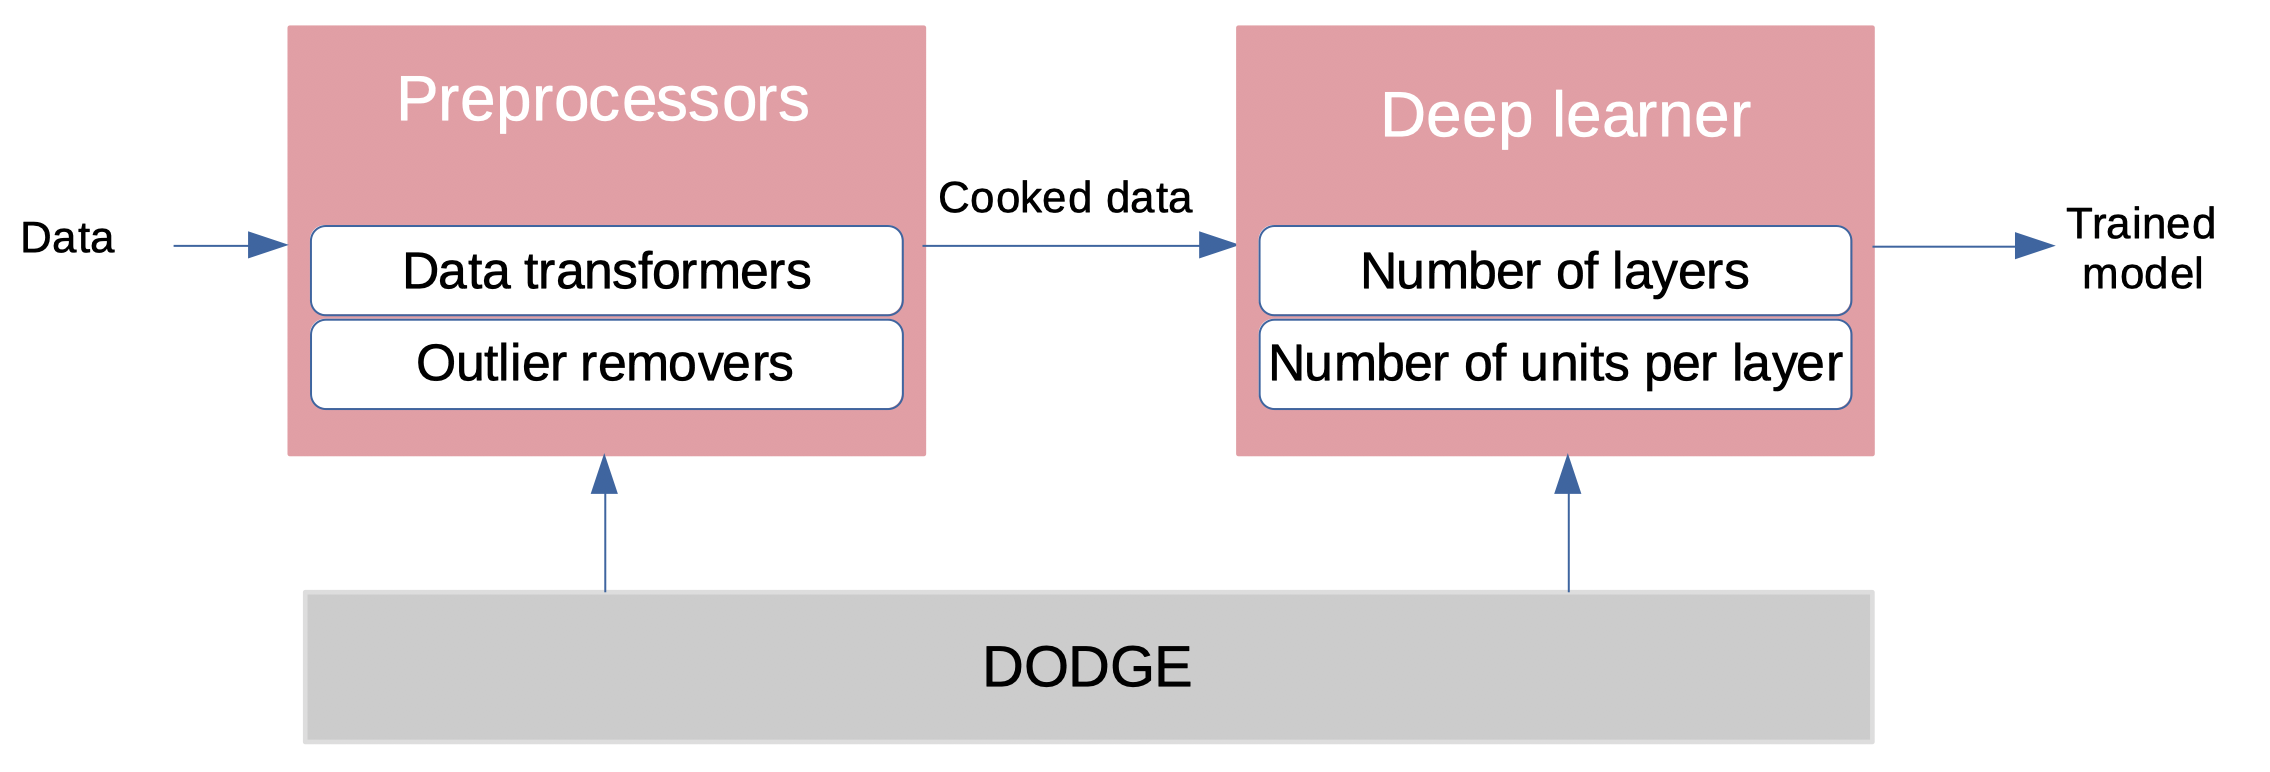
\includegraphics[width=\linewidth]{approach.png}
%     \caption{An overview of our approach. The blue boxes are various stages in the model development lifecycle. The white boxes inside are classes of hyperparameters to be tuned.}
%     \label{fig:approach}
% \end{figure}

% Figure \ref{fig:approach} offers an overview of our system. Raw data is preprocessed by a variety of methods, chosen by the hyperparameter optimizer (this is part of the search space). The result of the preprocessor(s), we call ``cooked" data. This is the data used by the deep learner, whose hyperparameters also we tune. Note that we use DODGE to tune both discrete and continuous hyperparameters. At the end is a trained model equipped with an optimized set of hyperparameters.

% We ran DODGE over three sets of hyperparameters: the preprocessors used (as discussed in Table \ref{tab:preprocessors}), the number of layers in the neural network, and the number of units per layer. The number of layers was constrained between $[1, 4)$, and the number of units per layer (each layer having the same number of units) was constrained to $[2, 20]$.

% Our choice for these bounds was not random: specifically, we used the results of Montufar et al. ~\cite{montufar2014number}; briefly, they discuss, for feedforward neural networks with ReLU activations (as we have used), bounds for the number of piecewise linear regions constituting a decision boundary that can be represented by a deep learner, providing a proof based on topological folding. In detail, when the number of units in any hidden layer is less than the number of inputs, the lower bound vanishes--this provided us with an upper bound for the number of units per layer (informally, while the network is still certainly capable of learning a complex decision boundary, it is no longer obliged to). To elaborate on this line of reasoning, given the results of their paper, it is trivial to show that an ideal neural network would have several layers, each with the same number of units (which in turn, is the same as the number of inputs)--this can be derived via a greedy algorithm that adds layers $l_i$ with the number of units as the number of inputs (denote this as $n_0$), until the remaining number of units (which can be trivially found from the results of the paper) is less than $2n_0$; at this point, we add one layer with the remaining number of units. While adding more units in the hidden layers certainly adds computational power, the formula presented in the paper suggests that deeper networks (in deep learning literature, ``deeper" denotes more layers) are preferable to ``wider" networks (which in deep learning literature refers to networks with more units in each layer). We made an assumption that no more than 3 layers with up to 20 units each would be required based on the formula presented in Montufar et al. ~\cite{montufar2014number}.


% \subsection{Neural network architectures}
%  Beyond this, we do not use other types of layers, since our approach is based on the kind of networks discussed by Montufar et al. ~\cite{montufar2014number}. Additionally, we voluntarily do not use Batch Normalization \cite{ioffe2015batch} based on the results of Santurkar et al. ~\cite{santurkar2018does}, who comment that batch normalization helps by flattening the loss surfaces (more precisely, it reduces the L-Lipschitzness and the $\beta$-smoothness of the loss surface), making optimization easier for gradient descent. We hypothesize that with our simple neural networks where the number of parameters is orders of magnitude less than the ones examined by them, that help is not strictly required, and simply using better optimization algorithms should suffice. We use the Adam \cite{kingma2014adam} optimizer in our experiments.


% Experimentally, we found that no more than 80 epochs were required for convergence. We test convergence by training using Early Stopping, which stops training if the validation loss does not improve after 5 epochs. The results of this test are shown in Figure \ref{fig:convergence}. However, our experiments use only 10 epochs. While we could have certainly gotten better results by running our learners for 80 epochs (and this would not have taken significantly longer), we wanted to demonstrate clearly that deep learners can achieve competitive performance very quickly, when used right and with proper tuning and choice of architectures (based off proven reasoning).





\section{Experimental Results}
\label{sec:results}

This rest of this paper uses the above methods to explore the research questions listed in
the introduction.

\subsection{Standard Deep Learning versus the Prior State-of-the-art ({\bf RQ1})}
\label{sec:rq1}



The results of this section address our {\bf RQ1} which was 
{\bf Does standard deep learning work for defect prediction?}.


Table \ref{tab:results} compares DL versus the prior state-of-the-art (DODGE) versus
our preferred new method (GHOST). {\bf RQ1} comments on the DL-vs-DODGE comparisons (and other comparisons are discussed, later in this paper).

 
In the 40 experiments of   Table \ref{tab:results}, DL only  performs  better than or the same as
DODGE in  10/40 experiments (see all the entries marked with ``*''). 
 A repeated patterns is that when DL wins on false alarm, it usually does so at the expense
 of low recalls.  Also,   when it does achieve a high recall (e.g. for velocity),
 this usually comes at the cost 
 of  high false alarms.
Hence we say:

% While for AUC, the baseline deep learning results (crafted by a human) outperform DODGE and GHOST for four datasets, those are the only cases (except in the case of pf on the lucene dataset) where GHOST does not outperform the baseline deep learning results. Clearly, we need to tune them for each metric. This failures of the baseline deep learners is particularly severe in the case of popt20 and recall.

\begin{blockquote}
    \noindent
    \BLUE
    For defect prediction, standard deep learners  are outperformed by existing state-of-the-art methods in 30/40 experiments. \BLACK
\end{blockquote}

 Note that these {\bf RQ1} results merely show that standard deep learning performs badly.
 Those results do not explain {\em why} that is so. For this task,
 we must move on to {\bf RQ2}.


\newcommand{\lightgray}[1]{\cellcolor{blue!7}\textcolor{black}{#1}}
\newcommand{\gray}[1]{\cellcolor{blue!20}\textcolor{black}{#1}}

\begin{table}[!t]
\caption{RQ1 results.
Cells show medians fo 20 runs.
Cells with an  "*" show the few
cases where DL
worked better than DODGE.
 \colorbox{blue!20}{Dark blue} shows  top rank (note: for pf, {\em less}
 is {\em better}), \colorbox{blue!7}{light blue} shows rank two;  white shows  lowest rank (worst performance). 
Rankings were calculated via
\S\ref{sec:dist}. The train and test versions used here are the same as the DODGE paper (see Table \ref{tab:datasets}).
}
\label{tab:results}
~~~~~~~~\begin{tabular}{ll|llll}
\toprule
                                         &       & AUC  & popt20 & recall & pf   \\ \midrule
\multicolumn{1}{l}{\multirow{3}{*}{ivy}} & DL &  0.58 & 0.15 & 0.33 & \gray{0.27} * \\
\multicolumn{1}{c}{}                     & DODGE & \gray{0.71} & \lightgray{0.25}   & \lightgray{0.85}   & \lightgray{0.36} \\
\multicolumn{1}{c}{}                     & GHOST & \lightgray{0.69}  & \gray{0.31}   & \gray{0.95}    & \lightgray{0.38} \\
\midrule \multirow{3}{*}{camel}          & DL & 0.55 & \lightgray{0.18} & 0.10 & \gray{0.04} *\\       
                                         & DODGE & \lightgray{0.58} & \gray{0.54}   & \lightgray{0.63}   & \lightgray{0.36} \\
                                         & GHOST & \gray{0.62} & \gray{0.54}   & \gray{0.65}   & 0.41 \\
\midrule \multirow{3}{*}{jedit}          & DL & 0.61 & 0.10 & 0.46 & \gray{0.16} *\\         
                                         & DODGE & \lightgray{0.63} & \lightgray{0.39}   & \lightgray{0.64}   & \gray{0.25} \\
                                         & GHOST & \gray{0.68} & \gray{0.41}   & \gray{0.91}   & \lightgray{0.40} \\
\midrule \multirow{3}{*}{log4j}          & DL & 0.55 & \lightgray{0.31} & 0.33 & \gray{0.13} *\\        
                                         & DODGE & \lightgray{0.61} & \gray{0.99}   & \lightgray{0.54}   & \lightgray{0.22} \\
                                         & GHOST & \gray{0.66} & \gray{0.99}   & \gray{0.75}   & \gray{0.19} \\
\midrule \multirow{3}{*}{velocity}       & DL & 0.50 & 0.57 & \gray{0.90} *& 0.87 \\         
                                         & DODGE & \lightgray{0.61} & \gray{0.64}   & 0.76   & \gray{0.47} \\
                                         & GHOST & \gray{0.68} & \lightgray{0.64}   & \lightgray{0.82}    & \gray{0.47}  \\
\midrule \multirow{3}{*}{synapse}        & DL & 0.54 & \lightgray{0.23} & 0.20 & \gray{0.05} *\\         
                                         & DODGE & \lightgray{0.65} & \gray{0.48}   & \gray{0.65}   & \lightgray{0.23} \\
                                         & GHOST & \gray{0.67} & \gray{0.48}   & \lightgray{0.63}   & 0.33 \\
\midrule \multirow{3}{*}{lucene}         & DL & 0.58 & \lightgray{0.51} & \gray{0.69} *& 0.52 \\         
                                         & DODGE & \gray{0.61} & \gray{0.80}   & \gray{0.67}    & \lightgray{0.36}  \\
                                         & GHOST & \lightgray{0.59} & \gray{0.80}   & \gray{0.7}   & \gray{0.34}  \\
\midrule \multirow{3}{*}{xalan}          & DL & 0.55 & \lightgray{0.24} & 0.21 & \gray{0.09} *\\        
                                         & DODGE & \lightgray{0.71} & \gray{1.0}    & \lightgray{0.71}   & \lightgray{0.14}  \\
                                         & GHOST & \gray{0.75} & \gray{1.0}    & \gray{0.76}   & 0.27 \\
\midrule \multirow{3}{*}{xerces}         & DL & 0.52 & \lightgray{0.28} & 0 & \gray{0.04} *\\         
                                         & DODGE & \lightgray{0.59} & \gray{0.93}   & \lightgray{0.54}   & \lightgray{0.15}  \\
                                         & GHOST & \gray{0.62} & \gray{0.94}   & \gray{0.57}   & 0.39 \\
\midrule \multirow{3}{*}{poi}            & DL & \lightgray{0.61} & 0.36 & \lightgray{0.45} & \gray{0.18} *\\         
                                         & DODGE & \gray{0.72} & \lightgray{0.66}   & \gray{0.78}   & \lightgray{0.22} \\
                                         & GHOST & \gray{0.73} & \gray{0.74}   & \gray{0.78}   & 0.38  \\
                                         \bottomrule
\end{tabular}
\end{table}
\begin{table}[!t]
    \centering
    \caption{RQ3 results. GHOST vs. DODGE. 
    Summary of Table~\ref{tab:results}.
    The first column indicates the number of wins, ties,  and losses  for each metric (these are defined using the $\Delta$ measure of Section \ref{sec:perfs} and the directions for ``better'' defined in Section \ref{sec:stats}.  Note that for popt20 and $pf$, there are multiple ties because both DODGE and GHOST achieve the highest possible score.}
  
  \scriptsize
   \begin{tabular}{rllll|r} 
   \toprule
    & AUC & Recall & popt20 & pf & Total \\
    \midrule
     \textbf{win} & 7 & 6 & 3 & 2 & 18 \\
    \textbf{tie} & 1 & 3 & 6 & 1 & 11 \\
     \textbf{loss} & 2 & 1 & 1 & 7 & 11 \\ \midrule 
     \textbf{win + tie} & 8 & 9 & 9 & 3 & 29 \\
     \bottomrule
    \end{tabular}
    \ 
    \label{tab:ghost_dodge}
\end{table}
\begin{table}[!t]
    \centering
    \caption{RQ3 results. GHOST vs. DL. Summary of Table~\ref{tab:results}. Same format as Table~\ref{tab:ghost_dodge}.}
    \scriptsize
   \begin{tabular}{rllll|r} 
   \toprule
    & AUC & Recall & popt20 & pf & Total \\
    \midrule
     \textbf{win} & 9 & 9 & 10 & 2 & 30 \\
     \textbf{tie} & 1 & 0 & 0 & 1 & 2 \\
     \textbf{loss} & 0 & 1 & 0 & 7 & 8 \\ \midrule 
     \textbf{win + tie} & 10 & 9 & 10 & 3 & 32 \\
     \bottomrule 
    \end{tabular}
    \ 
    \label{tab:ghost_dl}
\end{table}

 
 \subsection{Why Does Standard Deep Learning Fail? ({\bf RQ2})}
 \label{sec:rq2}
Our second research question was  {\bf RQ2} which was 
 {\bf Why does standard deep learning fail for defect prediction?}.
 Recall from Table~\ref{tab:datasets} that the class balance    between defective and non-defective modules is highly variable between our train and test sets.
 We conjecture that DL's failure to defeat tradition methods was that these algorithms were not
 tuned for such highly variable class balances.  Preliminary results with an artificially generated data set (recall Figures \ref{fig:unweighted} and \ref{fig:weighted}) showed that  unweighted loss functions
 means that a neural net can miss the  minority class.
 Those artificial results
 make us conjecture that:

 \begin{blockquote}
     \noindent
     The  lack of success  of  deep  learning  in  defect prediction  can  be  attributed  to  optimizing  for  the wrong performance metric.
 \end{blockquote}

This conjecture is tested in the next research question.

\subsection{  How to Fix Deep Learning? {\bf (RQ3)}}
\label{sec:rq3}

{\bf RQ1} assessed DODGE with respect to  standard DL. This checks if    GHOST  offers any added value over DODGE.
 

\begin{table*}[ht!]
\centering
\caption{Comparison of GHOST (optimized for recall) with the results of Wang et al. \cite{wang2016automatically} on within-project defect prediction. Bold indicates better results, as determined by point statistics ($0.3 \sigma = 4.91$).}
\label{tab:wpdp}
\begin{tabular}{l|ll|lll|lll|lll}
\toprule
Dataset & Train & Test & \multicolumn{3}{c}{ADTree PROMISE} & \multicolumn{3}{c}{Semantic} & \multicolumn{3}{c}{GHOST}    \\
\midrule
                         &                        &                       & P    & R    & F1                   & P    & R    & F1             & P    & R    & F1                \\
                         \midrule
\multirow{2}{*}{synapse} & 1                      & 1.1                   & 45.5 & 50   & 47.6                 & 46   & 66.7 & \cellcolor{blue!10}\textbf{54.4}           & 44.1 & 100  & \cellcolor{blue!10}\textbf{50.4}              \\
                         & 1.1                    & 1.2                   & 51.1 & 55.8 & 53.3                 & 57.3 & 59.3 & \cellcolor{blue!10}\textbf{58.3}           & 44.1 & 100  & \cellcolor{blue!10}\textbf{56.1}              \\
                         \midrule
\multirow{2}{*}{jEdit}   & 3.2                    & 4                     & 44.7 & 73.3 & 55.6                 & 46.7 & 74.7 & \cellcolor{blue!10}\textbf{57.4}           & 42.3 & 100  & \cellcolor{blue!10}\textbf{55.9}              \\
                         & 4                      & 4.1                   & 46.1 & 67.1 & 54.6                 & 54.4 & 70.9 & \cellcolor{blue!10}\textbf{61.5}           & 40.5 & 100  & 54.8              \\ \midrule
log4j                    & 1                      & 1.1                   & 49.1 & 73   & 58.7                 & 67.5 & 73   & \cellcolor{blue!10}\textbf{70.1}           & 55.6 & 100  & \cellcolor{blue!10}\textbf{65.9}              \\ \midrule
ivy                      & 1.4                    & 2                     & 22.6 & 60   & \cellcolor{blue!10}\textbf{32.9}                 & 21.7 & 90   & \cellcolor{blue!10}\textbf{35}             & 24.9 & 100  & \cellcolor{blue!10}\textbf{37.8}              \\ \midrule
\multirow{2}{*}{lucene}  & 2                      & 2.2                   & 73.3 & 38.2 & 50.2                 & 75.9 & 56.9 & 65.1           & 61.3 & 100  & \cellcolor{blue!10}\textbf{74.5}              \\
                         & 2.2                    & 2.4                   & 70.9 & 52.7 & 60.5                 & 66.5 & 92.1 & \cellcolor{blue!10}\textbf{77.3}           & 60.9 & 100  & \cellcolor{blue!10}\textbf{75.3}              \\ \midrule
\multirow{2}{*}{camel}   & 1.2                    & 1.4                   & 24.8 & 75.2 & 37.3                 & 96   & 66.4 & \cellcolor{blue!10}\textbf{78.5}           & 20.2 & 100  & 32.4              \\
                         & 1.4                    & 1.6                   & 28.3 & 63.7 & \cellcolor{blue!10}\textbf{39.1}                 & 26.3 & 64.9 & \cellcolor{blue!10}\textbf{37.4}           & 26.7 & 100  & \cellcolor{blue!10}\textbf{38.2}              \\ \midrule
xalan                    & 2.4                    & 2.5                   & 64.7 & 43.2 & 51.8                 & 65   & 54.8 & 59.5           & 62.7 & 100  & \cellcolor{blue!10}\textbf{66}                \\ \midrule
xerces                   & 1.2                    & 1.3                   & 16   & 46.4 & 23.8                 & 40.3 & 42   & \cellcolor{blue!10}\textbf{41.1}           & 18.6 & 100  & 30                \\ \midrule
\multirow{2}{*}{poi}     & 1.5                    & 2.5                   & 73.7 & 44.8 & 55.8                 & 76.1 & 55.2 & 64             & 72.2 & 100  & \cellcolor{blue!10}\textbf{83.2}              \\
                         & 2.5                    & 3                     & 75   & 75.8 & \cellcolor{blue!10}\textbf{75.4}                 & 81.6 & 79   & \cellcolor{blue!10}\textbf{80.3}           & 70.2 & 100  & \cellcolor{blue!10}\textbf{79.7}              \\ \midrule
\multirow{2}{*}{ant}     & 1.5                    & 1.6                   & 44.8 & 51.1 & 47.7                 & 88   & 95.1 & \cellcolor{blue!10}\textbf{91.4}           & 65.5 & 84.3 & 62.8              \\
                         & 1.6                    & 1.7                   & 41.8 & 77.1 & 54.2                 & 98.8 & 90.1 & \cellcolor{blue!10}\textbf{94.2}           & 52.6 & 99.4 & 57.3              \\
 \bottomrule
\end{tabular}
\end{table*}

\begin{table}[!b]
    \centering
    \caption{Comparison of GHOST with the results of Wang et al. \cite{wang2016automatically} on cross-project defect prediction. All results shown are F-1 scores. GHOST results are medians over 20 runs. Bold and \colorbox{blue!10}{dark blue} indicates better (in case of tie, both are in bold), as determined by point statistics
     of \S\ref{sec:point} (and here, 
    $0.3 \sigma = 4.41$).}
    \label{tab:tan}
    \begin{tabular}{ ll|ll }
    \toprule
	\textbf{Source} & \textbf{Target} & \textbf{Wang et al.} & \textbf{GHOST} \\
	\midrule
	jedit-4.1 & camel-1.4 & \cellcolor{blue!10}\textbf{69.3}  & 34.9 \\ 
	camel-1.4 & jedit-4.1 & \cellcolor{blue!10}\textbf{61.5}  & 47.3 \\ 
	lucene-2.2 & log4j-1.1 & \cellcolor{blue!10}\textbf{61.8}  & 51.7 \\ 
	xerces-1.3 & ivy-2.0 & \cellcolor{blue!10}\textbf{45.3} & 28.3 \\ 
	synapse-1.2 & ivy-2.0 & \cellcolor{blue!10}\textbf{82.4}  & 30.3 \\
	camel-1.4 & ant-1.6 & \cellcolor{blue!10}\textbf{97.9}  & 62.7 \\
	xalan-2.5 & xerces-1.3 & \cellcolor{blue!10}\textbf{38.6} & \cellcolor{blue!10}\textbf{35.7} \\ 
	ivy-2.0 & xerces-1.3 & \cellcolor{blue!10}\textbf{42.6} & \cellcolor{blue!10}\textbf{40.7} \\ 
	log4j-1.1 & jedit-4.1 & \cellcolor{blue!10}\textbf{50.3} & \cellcolor{blue!10}\textbf{49.4} \\ 
	jedit-4.1 & log4j-1.1 & \cellcolor{blue!10}\textbf{64.5} & \cellcolor{blue!10}\textbf{64.1} \\
	lucene-2.2 & xalan-2.5 & 55  & \cellcolor{blue!10}\textbf{65.4} \\ 
	xerces-1.3 & xalan-2.5 & 57.2 & \cellcolor{blue!10}\textbf{66} \\ 
	xalan-2.5 & lucene-2.2 & 59.4 & \cellcolor{blue!10}\textbf{73.8} \\ 
	log4j-1.1 & lucene-2.2 & 69.2 & \cellcolor{blue!10}\textbf{74.6} \\ 

	ivy-2.0 & synapse-1.2 & 43.3 & \cellcolor{blue!10}\textbf{60.9} \\ 
	poi-3.0 & synapse-1.2 & 51.4 & \cellcolor{blue!10}\textbf{58.1} \\ 
	synapse-1.2 & poi-3.0 & 66.1 & \cellcolor{blue!10}\textbf{82.7} \\ 
	ant-1.6 & camel-1.4 & 31.6 & \cellcolor{blue!10}\textbf{36} \\ 
	ant-1.6 & poi-3.0 & 61.9 & \cellcolor{blue!10}\textbf{77.8} \\ 
	poi-3.0 & ant-1.6 & 47.8 & \cellcolor{blue!10}\textbf{62.5} \\ 
	\bottomrule
\end{tabular}
    
\end{table}


\begin{table}[!b]
    \centering
    \caption{Summary of GHOST vs  Wang et al. \cite{wang2016automatically}}
    \label{tab:tan-summary}
    \begin{tabular}{l|ll|l}
    \toprule 
         & \textbf{WPDP (Tbl. \ref{tab:wpdp})} & \textbf{CPDP (Tbl. \ref{tab:tan})} & \textbf{Total} \\
         \midrule 
       win  & 3 & 10 & \textbf{13} \\
       tie  & 8 & 4 & \textbf{12} \\
       loss & 5 & 6 & \textbf{11} \\
       \midrule 
       \textbf{win + tie} & 11 & 14 & 25 \\
       \bottomrule
    \end{tabular}
\end{table}


Returning to
Table \ref{tab:results}, GHOST can be seen
to have more
 \colorbox{blue!20}{dark blue}
 cells than anything else (i.e. statistically, it is ranked number one most often).
Table~\ref{tab:ghost_dodge} and Table~\ref{tab:ghost_dl} summarize those results for comparison with DODGE:
\bi
\item
   18 times, GHOST defeats DODGE (see top-right, Table \ref{tab:ghost_dodge});
\item
  29 times, GHOST defeats  DL (see top-right, Table \ref{tab:ghost_dl});\item
  11 times, GHOST was as good as DODGE (see mid-right,  Table \ref{tab:ghost_dodge})
\ei
Tables~\ref{tab:results}, \ref{tab:ghost_dodge}, \ref{tab:ghost_dl} display
distribution results where algorithms  were run multiple times using different random number seeds.
Tables   \ref{tab:wpdp}
and \ref{tab:tan},
on the other hand,
show display
point distribution results were our algorithms are compared to the single set of
performance points
reported in prior work.


This is also seen in comparison with the results of Wang et al., where we perform as good or better in 11/16 datasets for within-project defect prediction. In cross-project defect prediction, we also note that we win 10/20 times and tie 4/20 times; this suggests that GHOST may be able to generalize well across different projects.

Table \ref{tab:tan-summary} summarizes the comparison with the results of Wang et al. \cite{wang2016automatically}.
\bi
    \item For within-project defect prediction (WPDP), GHOST (tuned for recall) defeats a Deep Belief Network (DBN) 3 times, ties 8 times, and loses 5 times. This suggests that tuning for recall does not necessarily lead to better F-1 scores (but does lead to better recalls).
    \item For cross-project defect prediction (CPDP), GHOST (tuned for F-1 score) defeats DBN-CP 9 times, ties 5 times, and loses 6 times.
    \item We note here that GHOST performs far better for cross-project defect prediction (10/14 = 71.4\% wins vs. 3/11 = 27.3\% wins). This could be indicative of strong generalizing ability of GHOST.
    \item
    \BLUE
    We observe that GHOST is matched or outperformed by Wang et al.'s approach in 13/16 cases. This, coupled with the previous observation, leads us to believe that GHOST is better suited to cross-project defect prediction (i.e., more general predictions) than within-project defect prediction. Nevertheless, GHOST remains a fast approach in all settings, completing hyperparameter optimization in a few minutes (see RQ5).
    \respto{2a2.1}
    \BLACK
\ei

These results recommend GHOST over DODGE and DBN. Also, they 
 deprecate the use of off-the-shelf standard DL for defect prediction (since GHOST clearly is preferred to standard DL). We attribute the super performance of GHOST to its weighted loss function.

The exceptions to the above pattern are the  GHOST vs DODGE recall results, which we will discuss in the next section.
Apart from that, we say that:

\begin{blockquote}
    \noindent
    For most evaluation goals, this modified version of deep learning performs better than the prior state-of-the-art.
\end{blockquote}

 
%  It is insightful to reflect on the impact of the weight schemes for different performance measures.
%  For AUC, using  $w_i > 1$ proved
%  {\em disadvantageous} since  AUC takes into account false positives as well. Notice that although in the last three datasets, the baselines had the best performance, the deep learners with $w_i =1$ dowa still out-perform (in the case of lucene), or match  performance (in jEdit and poi) with DODGE.
%  But for $1-pf$,  $w_i > 1$ proved  {\em advantageous} since, here, we seek the reverse property (where we want to avoid positive results).
 
 
%  Best results were found using a weight control parameter of $w_i=1$ for AUC, recall pot20 and 
%  $w_i=10$ for $1-pf$. 
 
%  These different results from different weights could be used to say  that we need to run the 
%  optimization with different weights for different goals.  But we do not recommend that.
%  Figure~\ref{fig:pf}  shows that, usually, the $(1-pf)$ results are all very similar. Hence, on pragmatically,   would argue that $w_i=1$ is a useful default.
 
%  The fact that our baseline deep learners beat baseline DODGE (and in two cases, outperform our weighted deep learner) is not necessarily surprising: after all, the baseline was crafted using the recommendations from deep learning literature \cite{montufar2014number}. We therefore state these results as cases where a human-designed deep learner outperforms one chosen by DODGE. Nevertheless, our weighted learner do match or outperform the baseline DODGE results, and in other datasets improves upon the baseline deep learning results, which emphasizes the importance of tuning the loss function correctly.
 

 
 



% For popt20, we ran the networks with a weight of 1, and found that there was no dataset where our results were statistically significantly worse than DODGE, so we did not proceed further. Note that for log4j, xalan, and xerces, the popt20 values are already high--we match the results of DODGE, which already achieves outstanding performance. Our popt20 results exemplify our core argument: it is important to tune the optimization goal of deep learners to match user goals. While our baseline deep learners, which were untuned and therefore optimize for accuracy, do worse in \textit{all} the datasets, our tuned deep learners significantly improve upon them, and do not lose in \textit{any} dataset.

% We ran the networks with a weight of 10 for false positive rate (pf), and found that GHOST performs well in all datasets, beating DODGE in 3 (lucene, poi, jEdit). Because so many of the values are 0, and therefore would not show up in the plots, we report 1 - pf values, so that higher values are better. We find that GHOST outperforms or matches DODGE in all datasets.

% We were unable to optimize GHOST for recall (see Figure \ref{fig:recall}). Running for 80 epochs rather than 10 also did not improve our results. We therefore conclude that deep learning is not a panacea; while deep learning can be optimized for many goals, it cannot be optimized for \textit{all} of them.


\subsection{Use Deep Learning in All Cases? (RQ4)}
\label{sec:rq4}

The results of this section address our \textbf{RQ4} which was \textbf{Does deep learning work well in all cases?}.

The false alarm rate results for GHOST in Table \ref{tab:results}, while respectable, loses to DODGE.  Note that we made considerable efforts to improve the results (e.g. weighted fuzzy oversampling, SMOTE, optimizing for different metrics), to no avail.
 Hence we offer the following:
 \bi
 \item
 In domains where the goal  is to ``cut corners''
 to find the most defects with the least effort, then we want to optimize for popt20 (since that criteria leads us to models that find most bugs with least inspection effort). In those domains, the results of Table~\ref{tab:ghost_dodge}  recommend DL with GHOST
 \item Our results also lend support to using GHOST in systems where raising false alarms is less disastrous than missing a true positive (recall).
 \BLUE
 \item In other domains where it is mission critical to raise few false alarms, then the results shown in Table~\ref{tab:ghost_dodge} show us that DODGE, rather than GHOST (or DL) may be better. 
 \BLACK
 \ei
Hence we say: 
 
 
% By examining our results in Figures \ref{fig:auc} - \ref{fig:recall}, we observe the general trend that GHOST outperforms our baseline deep learners and DODGE. However, this is only true for 3 out of 4 metrics: in recall, DODGE outperforms GHOST on most datasets. The humbling result then, is that while deep learners can, in many cases, prove to be excellent candidates for learners, they must be evaluated against classical machine learning models in view of the goal to be optimized for.


\begin{blockquote}
    \noindent
    We recommend the use of deep learning in domains where false alarms are not particularly catastrophic.
\end{blockquote}

\subsection{Scalability of Deep Learning (RQ5)}
\label{sec:rq5}

\begin{wraptable}{r}{1.8in}
    \centering
    \caption{Median training time over 20 repeats.}
    \scriptsize
    \begin{tabular}{rll}
        \toprule
          & Training   & GHOST   \\
           &   (secs) &  (secs) \\
        \midrule
        ivy & 0.78 & 9m 17s \\
        lucene & 0.81 & 10m 26s \\
        poi & 1.09 & 13m 44s \\
        synapse & 0.81 & 9m 48s \\
        velocity & 0.88 & 10m 20s \\
        camel & 1.41 & 18m 10s \\
        jEdit & 1.11 & 14m 32s\\
        log4j & 0.73 & 8m 29s\\
        xalan & 1.61 & 20m 16s\\
        xerces & 1.08 & 11m 56s \\
        \bottomrule \\
    \end{tabular}
    \label{tab:runtimes}
\end{wraptable}The results of this section address \textbf{RQ5} which was \textbf{How slow is tuning for deep learning for defect prediction?}.

To answer this question, we report the median training time over 20 runs. The measured time is CPU time, when trained on a 4-core Intel Core i5 CPU. These are summarized in Table \ref{tab:runtimes}. Clearly, our models are very fast (less than 2 seconds to train on a CPU).

Table \ref{tab:runtimes} also shows the runtimes for running GHOST on different datasets. Because GHOST runs 20 times to find the median value of a metric, the runtimes we report are for all 20 runs. However, we do not divide this time by 20 as we feel it is scientifically important to run a stochastic experiment multiple times and report statistical results.

Figure \ref{fig:scalability} shows our scalability results, which we obtain by measuring the training time for different sizes of the datasets.
We observe a general trend across all datasets that deep learning scales well with the size of the problem. More specifically,  GHOST's runtimes grows sublinearly. For example, in the xalan results:
\bi
\item A 500\% increase in data   (from a fifth to all the data)...
\item ... leads to a runtime increase of   only    $2.7/1.5 = 180\%$.
\ei

Hence we say: 
\begin{blockquote}
    \noindent
    Tuning deep learners is both practical and tractable for defect prediction.
\end{blockquote}



\begin{figure}[!t]
    \centering
    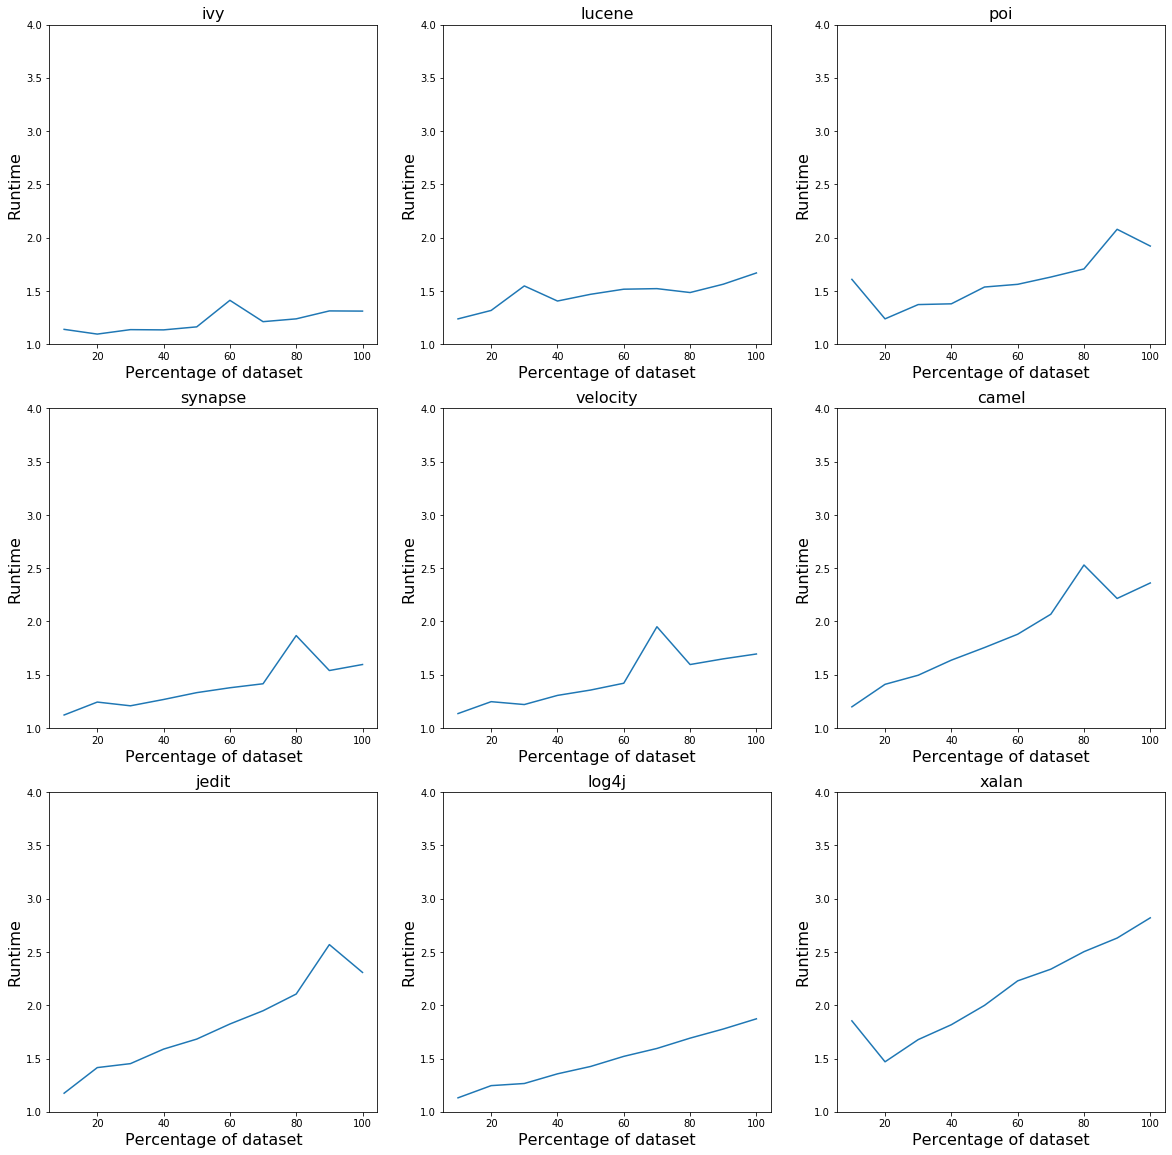
\includegraphics[width=\linewidth]{scalability.png}
    \caption{Scalability results for 9 datasets. The x-axis is the perentage of the dataset trained on; the y-axis is the runtime in seconds on a CPU.}
    \label{fig:scalability}
\end{figure}

\section{Threats to Validity}
\label{sec:threats}
 
 
\textbf{Sampling bias:} As with any other data mining paper, it is important to discuss sampling bias. We claim that this is mitigated by testing on 10 SE projects over multiple versions, and demonstrating our results across all of them. Nevertheless, in future work, it would be useful to explroe more data. 

\textbf{Learner bias:} Our learner bias here corresponds to the choice of architectures we used in our deep learners. As discussed above, we chose the architectures based on our reading of ``standard DL'' from the literature. That said, different DL architectures could lead to different results.

\textbf{Evaluation bias:} We compared our methods using a range of   metrics: AUC, recall, false alarm rate, and popt20. We used these  varied evaluation metrics to demonstrate more clearly the benefits of not using learners off-the-shelf, and tuning the loss function optimized. If other performance metrics are used, then other results might be obtained.

\textbf{Order bias:} This refers to bias in the order in which data elements appear in the training and testing sets. We purposely choose these so that the testing set is from a newer version than the data used in the training set, following the natural order of software releases. Therefore, we argue that such a bias is needed to mimic real-world usage of such learners.

\textbf{External validity:} We tune major hyperparameters using DODGE, removing external biases from the approach. Our baseline results are based on the results of Montufar et al. ~\cite{montufar2014number}, which has been evaluated by the deep learning community.

\section{Conclusion}
\label{sec:conclusion}

This paper has argued:

 \begin{blockquote}
    \noindent
    For SE,  do not use   off-the-shelf  deep learning. 
  Instead,
tune that algorithm to the needs of SE (using tools like, e.g. GHOST).
\end{blockquote}
To make that case, this paper explored   GHOST, a new method that combines deep learning
and the $\epsilon$-domination heuristic with a set of tweaks: (a) weighted loss functions (see \S\ref{sec:loss}) (b) weighted fuzzy oversampling (see \S\ref{sec:wfo}) (c) SMOTE \cite{Chawla02}, an oversampling method.
 We demonstrated the efficacy of our approach on 10 defect prediction datasets, using four metrics. We compared our results against two sets of baselines, one being a reasonable baseline based off deep learning research and prior state-of-the-art result in defect prediction, and the other being a prior result using deep learning to extract features from code.  
 We presented scalability and runtime tests to demonstrate that deep learners can be trained quickly.
We showed that best results come from  learners properly tuned for the dataset and the goal metric (using a weighted loss function). 
 
Finally, we note that one could apply the weighted loss functions to classical learners, such as support vector machines (SVMs), which rely on an optimization setup.

% In addition, we make a case for critically evaluating learners against prior work, and in particular, comparing deep learning results against non-deep learning results. In a domain where active learning is increasingly popular, it is vital for a learner to have rapid training times, and our approach demonstrates that deep learners need not be eliminated from consideration without a fair chance. The principles we present in this paper, then, can be summarized succinctly as follows:

% \begin{blockquote}
%     \textit{Learners must be guided towards a goal, tuned using hyperparameter optimization, with as simple architectures as possible, to save time.}
% \end{blockquote}

% Finally, we comment on potential improvements in the future. One potential avenue is to use better optimizers, especially those exploiting the topology of the loss surface. Such advanced optimization techniques are heavily studied in the deep learning literature.
 

 We take  care to stress that our results on relate to defect prediction. As to other areas of software analytics, that is a matter for future search. That said,
our results suggest that, for future work, the following research agenda could be insightful:
 \begin{enumerate}
\item
 Divided analytics into various domains. 
 \item
 Then, for each domain:
 \begin{enumerate}\item
 Determine the prior non-DL state-of-the-art; \item Compare DL with that state-of-the-art; 
 \item Seek ways to better adapt DL to that domain.
 \end{enumerate}\end{enumerate} 
 
 
\section*{Acknowledgements}
This work was partially funded by 
a research grant from the National Science Foundation (CCF \#1703487).

\balance
\bibliographystyle{IEEEtran}
\bibliography{cite} 

\begin{minipage}{.5\textwidth}
% biography
\begin{IEEEbiography}[{
\includegraphics[width=1.05in,clip,keepaspectratio]{rahul.jpeg}}]{Rahul Yedida} is a first-year PhD student in Computer Science at NC State University. His research interests include automated software testing and machine learning for software engineering. For more information, please visit \url{https://ryedida.me}.
\end{IEEEbiography}
 

\begin{IEEEbiography}[{
\includegraphics[width=1.05in,clip,keepaspectratio]{menzies.png}}]{Tim Menzies} (IEEE Fellow, Ph.D. UNSW, 1995)
is a Professor in comptuer science  at NC State University, USA,  
where he teaches software engineering,
automated software engineering,
and programming languages.
His research interests include software engineering (SE), data mining, artificial intelligence, and search-based SE, open access science. 
For more information,  please visit \url{http://menzies.us}.
\end{IEEEbiography}
\end{minipage}

%%%%%%%%%%%%%%%%%%%%%%
% REVIEWER RESPONSES %
%%%%%%%%%%%%%%%%%%%%%%

\appendices 
\clearpage

\setcounter{page}{1}
\pagenumbering{roman}
\normalsize
\twocolumn
% \newpage
% \twocolumn
\section*{Response to Reviewers}
\subsection*{Response to AE}

{\em Thank you for submitting to TSE.  The reviewers have now finished their reviews of the paper.  I am recommending that the authors produce a major revision based on these reviews, which the reviewers will re-review and make a final decision on. }

Thank you for this opportunity to revise this paper. We wish to thank the reviewers for their careful and insightful comments. Typos are fixed  and readability is improved with careful proof-reading. And we have revised the draft according to reviewer comments. (shown as \respto{1a(1-4)}, \respto{2a(1-4)} and \respto{3a(1-5)}, respectively). All changed text is highlighted in \textcolor{blue}{blue}.
% TODO: Change above.

{\em The reviewers' two main concerns are with (1) the evaluation sometimes being based on what they deemed to be anecdotal evidence, and generally not organized and supported as well as it should be;} 

\BLUE
We would like to thank the reviewers for their critical evaluation of our paper. We have provided more concrete evidence to support our claims in the text to address this concern.
\BLACK

{\em and (2) a need for a stronger explanation of the unique contributions of this approached, as compared to prior approaches.}

\BLUE
We have revised the text to emphasize more clearly our contributions in the paper, highlighting the key advantages of our approach over prior work.
\BLACK

{\em The reviewers are clearly not yet convinced that this paper warrants publication, though they agree that the problem is important and the approach has merit, so I warn caution that, if the revision is submitted, the reviewers may still decide against accepting this paper. There is a split, with grounded concerns, between asking for a revision and rejecting but allowing the authors to resubmit as new. My judgement came out on the more positive side of hoping the revision can address the concerns satisfactorily, though, again, I urge caution.}

\BLUE
We appreciate your support for this paper. We hope our revisions bring our paper to an acceptable standard for the reviewers.
\BLACK

\subsection*{Response to Reviewer \#1}

{\em {\bf R1-a:} It’s not clear what is the unique contribution of GHOST to software engineering tasks such as defect prediction when being applied on DL for hyperparameter tuning since these kind of parameter tuning methods can be applied to any DL algorithms in general and they had been applied in image processing domain.}

\respto{1a1}
\BLUE
 We agree that our text did not sufficiently demonstrate the specific usefulness of our approach to software engineering problems. At this point, we did not believe we had sufficient evidence to make a more general claim than to comment that GHOST works for defect prediction; it would have been speculative at best to assume the same approach would work in other domains.

While oversampling is certainly well studied in deep learning literature (we point the reader to Buda et al. \cite{buda2018systematic} for a recent practical review), our approach is tailored to defect prediction in the following ways: (a) it is natural to expect a class imbalance in a defect prediction dataset (or at least, one would hope so); therefore, GHOST outperforms prior work in defect prediction because it is tailored to the specific nature of defect prediction datasets (b) further, we note that as shown recently by Agrawal et al. \cite{agrawal2020simpler}, DODGE works well in software engineering, but not in non-SE domains due to the more complex nature of the data. We therefore do not expect GHOST to work in such domains either, because the underlying hyperparameter optimizer is DODGE.
\BLACK

{\em {\bf R1-b:} Can you explicitly define what is a standard DL architecture for defect prediction?
Since the features (static attributes) in table 4 that are taken into account by the DL algorithms are all code attributes, the paper title can be descoped to only code defects or bug prediction.}

\respto{1a2}
\BLUE
You are correct that we did not concretely define what ``standard" deep learners are. We have added a precise definition to our text \citeresp{1a2.1}. For clarity, we repeat this definition here. A ``standard" deep learner in our paper means an untuned deep learner, whose hyperparameters are derived from deep learning literature. Specifically, for our comparison study, we use the results of Montufar et al. \cite{montufar2014number} to design an architecture. Briefly, their results can be inferred as: by maintaining the number of nodes in the hidden layers to be at least the number of inputs, the network has a nonzero lower bound on the number of piecewise linear regions in its decision boundary. Although this does not necessarily mean a ``better" decision boundary, it does imply some effort by the deep learner to find an optimal boundary.

While GHOST is trained on static code attributes, we note that our results still outperform more sophisticated, text-based features as derived by Wang et al. \cite{wang2016automatically} (see Table \ref{tab:tan-summary}). Further, we attempted to obtain the semantic features used by Wang et al. in their study, but they could not share the data due to the proprietary nature of their work; this limited us to use data we had on the software versions they mined. However, we maintain that GHOST will work on any defect prediction dataset that has a class imbalance problem.
\BLACK

{\em {\bf R1-c:} In Weighted Fuzzy Oversampling, can you explain how delta r and training data is generated in defect prediction using a specific example? How will weighted fuzzy oversampling improve the performance of defect prediction?
}

\respto{1a3}
\BLUE
Thank you for your comments. We agree that the discussion of the use of weighted fuzzy oversampling in GHOST deserved more elaboration. As discussed in \S \ref{sec:wfo}, $\boldsymbol \Delta \textbf{r}$ is set to a fixed value (more precisely, a vector whose each value) is between 0.05 and 0.1. In \S \ref{sec:pseudocode}, we discussed the utility of each component of GHOST; we have since updated this discussion to include a more complete explanation of the reasoning behind using weighted fuzzy oversampling \citeresp{1a3.1}. For completeness, we also copy the added text below.

Weighted loss functions perform standard oversampling in a computationally efficient way, balancing out the classes. However, it achieves this efficiency by weighting each minority class sample more. Therefore, the deep learner can, in theory, still reduce the value of this loss function by narrowly classifying the minority samples correctly. This behavior is undesired because it is, essentially, overfitting on part of the learner, since it only adjusted the decision boundary based on the training data. Weighted fuzzy oversampling is an attempt to alleviate this issue by adding ``guard points" around the minority class point, further pushing away the neural network decision boundary. That said, we do not wish to ``pollute" the original training data with fake data points, and so we reduce the ``value" (where value means the loss function value) of these points with the exponential decay (the $2^i$ in the denominator).

Finally, with the extra added points, the data is now unbalanced the other way, and we fix this with a well-known oversampling strategy, SMOTE.
\BLACK

{\em {\bf R1-d:} Table 9 is confusing. It seems that Wang et. al wins 11/20 times in terms of F1 measures using deep learning generated “Semantic” features to train a Naive Bayes model on within-project defect prediction. In certain datasets such as xerces and ant, Wang et. al performs significantly better than GHOST. Most of the remaining 9 wins of GHOST is marginal. Can you explain why?
}

\respto{1a4}
\BLUE
You are correct in your interpretation of the results. It is difficult to give a clear explanation about why this phenomenon occurs, and any explanation would at best be an educated guess, since the decision boundaries are high-dimensional. Our educated guess here, is that the data samples in the training data are mixed to the point where GHOST either (a) cannot distinguish between the classes as well as the semantic features, (b) worsens this mixing problem through weighted fuzzy oversampling, or (c) missed an optimal hyperparameter configuration, either due to optimizing for recall, or for not running for enough iterations.

We comment here that, as seen in Table \ref{tab:tan-summary}, while GHOST does lose to Wang et al. in within-project defect prediction, it does much better in cross-project defect prediction. On seeing Table \ref{tab:tan} (the cross-project defect prediction results), we see a similar imbalance in favor of both sides (in particular, we note the pairs (a) jedit-camel in favor of Wang et al. (b) synapse-ivy in favor of Wang et al. (c) camel-ant in favor of Wang et al. (d) xalan-lucene in favor of GHOST (e) synapse-poi in favor of GHOST (f) poi-ant in favor of GHOST). Again, we cannot precisely explain \textit{why} this phenomenon occurs, only that it happens at all (with our educated guess above).
\BLACK

\subsection*{Response to Reviewer \#2}

{\em {\bf R2-a:} RQ1 is ``Does standard deep learning work for defect prediction?". I find the answer to this question (``For defect prediction, standard deep learners do not perform better than existing state-of-the-art methods in 30/40 experiments") ambiguous and unconvincing even though the results clearly indicate that DODGE outperforms the standard technique in most cases. I am only suggesting a better explanation or rewording here. Consider a situation in which the standard DL outperforms DODGE in 10 experiments and does equally well in all remaining 30 cases. Your answer does not contradict with this situation but the conclusion ``Note that these RQ1 results merely show that standard deep learning performs badly." no longer holds.}

\respto{2a1}
\BLUE
Thank you for pointing this out with the elaborate example. We now realize the lack of specificity in our original RQ1 answer, and have updated it to reflect the exact scenario \citeresp{2a1.1}.
\BLACK

{\em {\bf R2-b:} Section 4.3 is the biggest concern. This subsection is not well-written and is misleading too. a) It doesn't say clearly that Wang et al. technique is better or equally good in 13/16 data sets for within-project defect prediction.}

\respto{2a2}
\BLUE
You are correct that Wang et al.'s approach is better than or equally good as GHOST for within-project defect prediction in 13/16 cases. Although this can be inferred from Table \ref{tab:tan}, we understand how the lack of explicit discussion on this is suspicious. We have addressed this in a new paragraph in the same subsection, discussing how GHOST is better suited to the cross-project scenario \citeresp{2a2.1}. In addition, we note that in the within-project case, GHOST was optimized for recall rather than F-1 score, strengthening our core idea that deep learners should be tuned to the desired metric.
\BLACK

{\em {\bf R2-c:} The authors' say ``In cross-project defect prediction, we also note that we win 9/20 times and tie 5/20 times". However, if I take a look at Table 10, I think the win is in 10 cases and the tie is in 4 cases. Am I misinterpreting the results?}

\respto{2a3}
\BLUE
Thank you for pointing out this error. Your interpretation is correct, and we have fixed the error in the text.
\BLACK

{\em {\bf R2-d:} This discussion does not say explicitly that in all remaining 10 cases where GHOST does not win, Wang et al.'s approach ends up performing better albeit only marginally in 4 cases that have been defined as ``tie". I am not challenging the definition of ``tie" but the fact still remains that those numbers are still in favour of Wang et al. Therefore I am not convinced with the authors' claim that ``For most evaluation goals, this modified version of deep learning performs better than the prior state-of-the-art." As a consequence, the generalizability claim about GHOST is also not convincing. To make a more convincing case, I suggest more benchmarks to be included to address this question. Alternatively, please provide a better explanation if my understanding is incorrect.
}

\respto{2a4}
\BLUE
TODO
\BLACK

{\em {\bf R2-e:} The paper mentions that ``For within-project defect prediction (WPDP), GHOST (tuned for recall) defeats a Deep Belief Network (DBN) 3 times, ties 2 times, and loses 5 times." If I take a look at Table 9, I see ties 8 times. Am I misinterpreting the results? Moreover, in 11 out of 16 cases Wang et al.'s approach has higher F-1 scores. In at least 5 cases the score is considerably better than GHOST's. Therefore, I find the results quite inconsistent with the authors' claim at the end.
}

\respto{2a5}
\BLUE
Thank you for pointing out this error. We have updated the text to reflect 8 ties instead of 2. To address the second part, we note that while the numbers in Table \ref{tab:tan} are better in the case of Wang et al. 11/16 times, they are median values, and for that reason, we do not recommend comparing the raw numbers. Instead, we choose to use statistical tests (in this case, Cohen's d test (see Section \ref{sec:stats} for a justification on the choice of test) to compare a distribution (our results) to a point estimate (Wang et al.). This is necessary to account for the inherent stochastic nature of deep learners stemming from random weight initialization.
\BLACK

{\em {\bf R2-f:} Please define m, i, $c_0$ and i$\Delta r$ in Algorithm 1 itself for more convenient reading.
}

\respto{2a6}
\BLUE
Thank you for pointing out that our notation was not discussed. We have corrected this by adding in a relevant subsection before the discussion of the algorithm \citeresp{2a6.1}.
\BLACK

\end{document}
